\chapter{Appendices}

\section{Life quality as walkability}

\subsection{Secondary data sources}
\label{SI:walkabilityData}
\begin{itemize}
  \item {Sport associations in Budapest}~\cite{HU_sport}
  \item {Kindergartens, daycares, primary and secondary education}~\cite{HU_Edu}
  \item {Art and music schools}~\cite{HU_Art}
  \item {Child health services}~\cite{HU_Child}
  \item {Social welfare system (eg.: elderly care)}~\cite{HU_Social}
  \item {Culture centers}~\cite{HU_Cult}
  \item {Indoor playgrounds}~\cite{HU_Play}
  \item {Healthcare (hospitals, private and public clinics, specialists)}~\cite{HU_Health}
  \item {Fitness and training facilities}~\cite{HU_Fitness}
  \item {Outdoor fitness facilities}~\cite{HU_outfitness}
  \item {Thermal baths and spa}~\cite{HU_Thermal}
  \item {Playgrounds and parks}~\cite{HU_Park}
\end{itemize}

\subsection{Weights used in the calculations}
The weights of the different $Q$ indices in the final aggregation as well as in sub-categories highly depends on the context and the nature of the problem. Here we present the values we used to generate the results of this study, that were agreed upon consulting with experts.

% The weights of the sub-indices from equation (\ref{final_Q}) are of the following values:
% \begin{itemize}
%   \item $w^{\text{services}}=0.7$;
%   \item $w^{\text{safety}}=0.1$;
%   \item $w^{\text{environment}}=0.2$
% \end{itemize}

The category weights used in equation (\ref{Q_services}), aggregating $Q^{services}$ are:

\begin{itemize}
  \item $w^{\text{family}}= 0.3$;
  \item $w^{\text{health}}= 0.3$;
  \item $w^{\text{culture}} = 0.15$;
  \item $w^{\text{sport}} = 0.15$;
  \item $w^{\text{night life}}=0.1$
\end{itemize}

\section{Data-driven strategies for optimal bicycle network growth}
\subsection{Data}

Figure \ref{fig:Nodes} shows the connected component size distribution $P(N_{cc})$ for all considered layers and cities.

\begin{figure*}[h!]
  \centering
  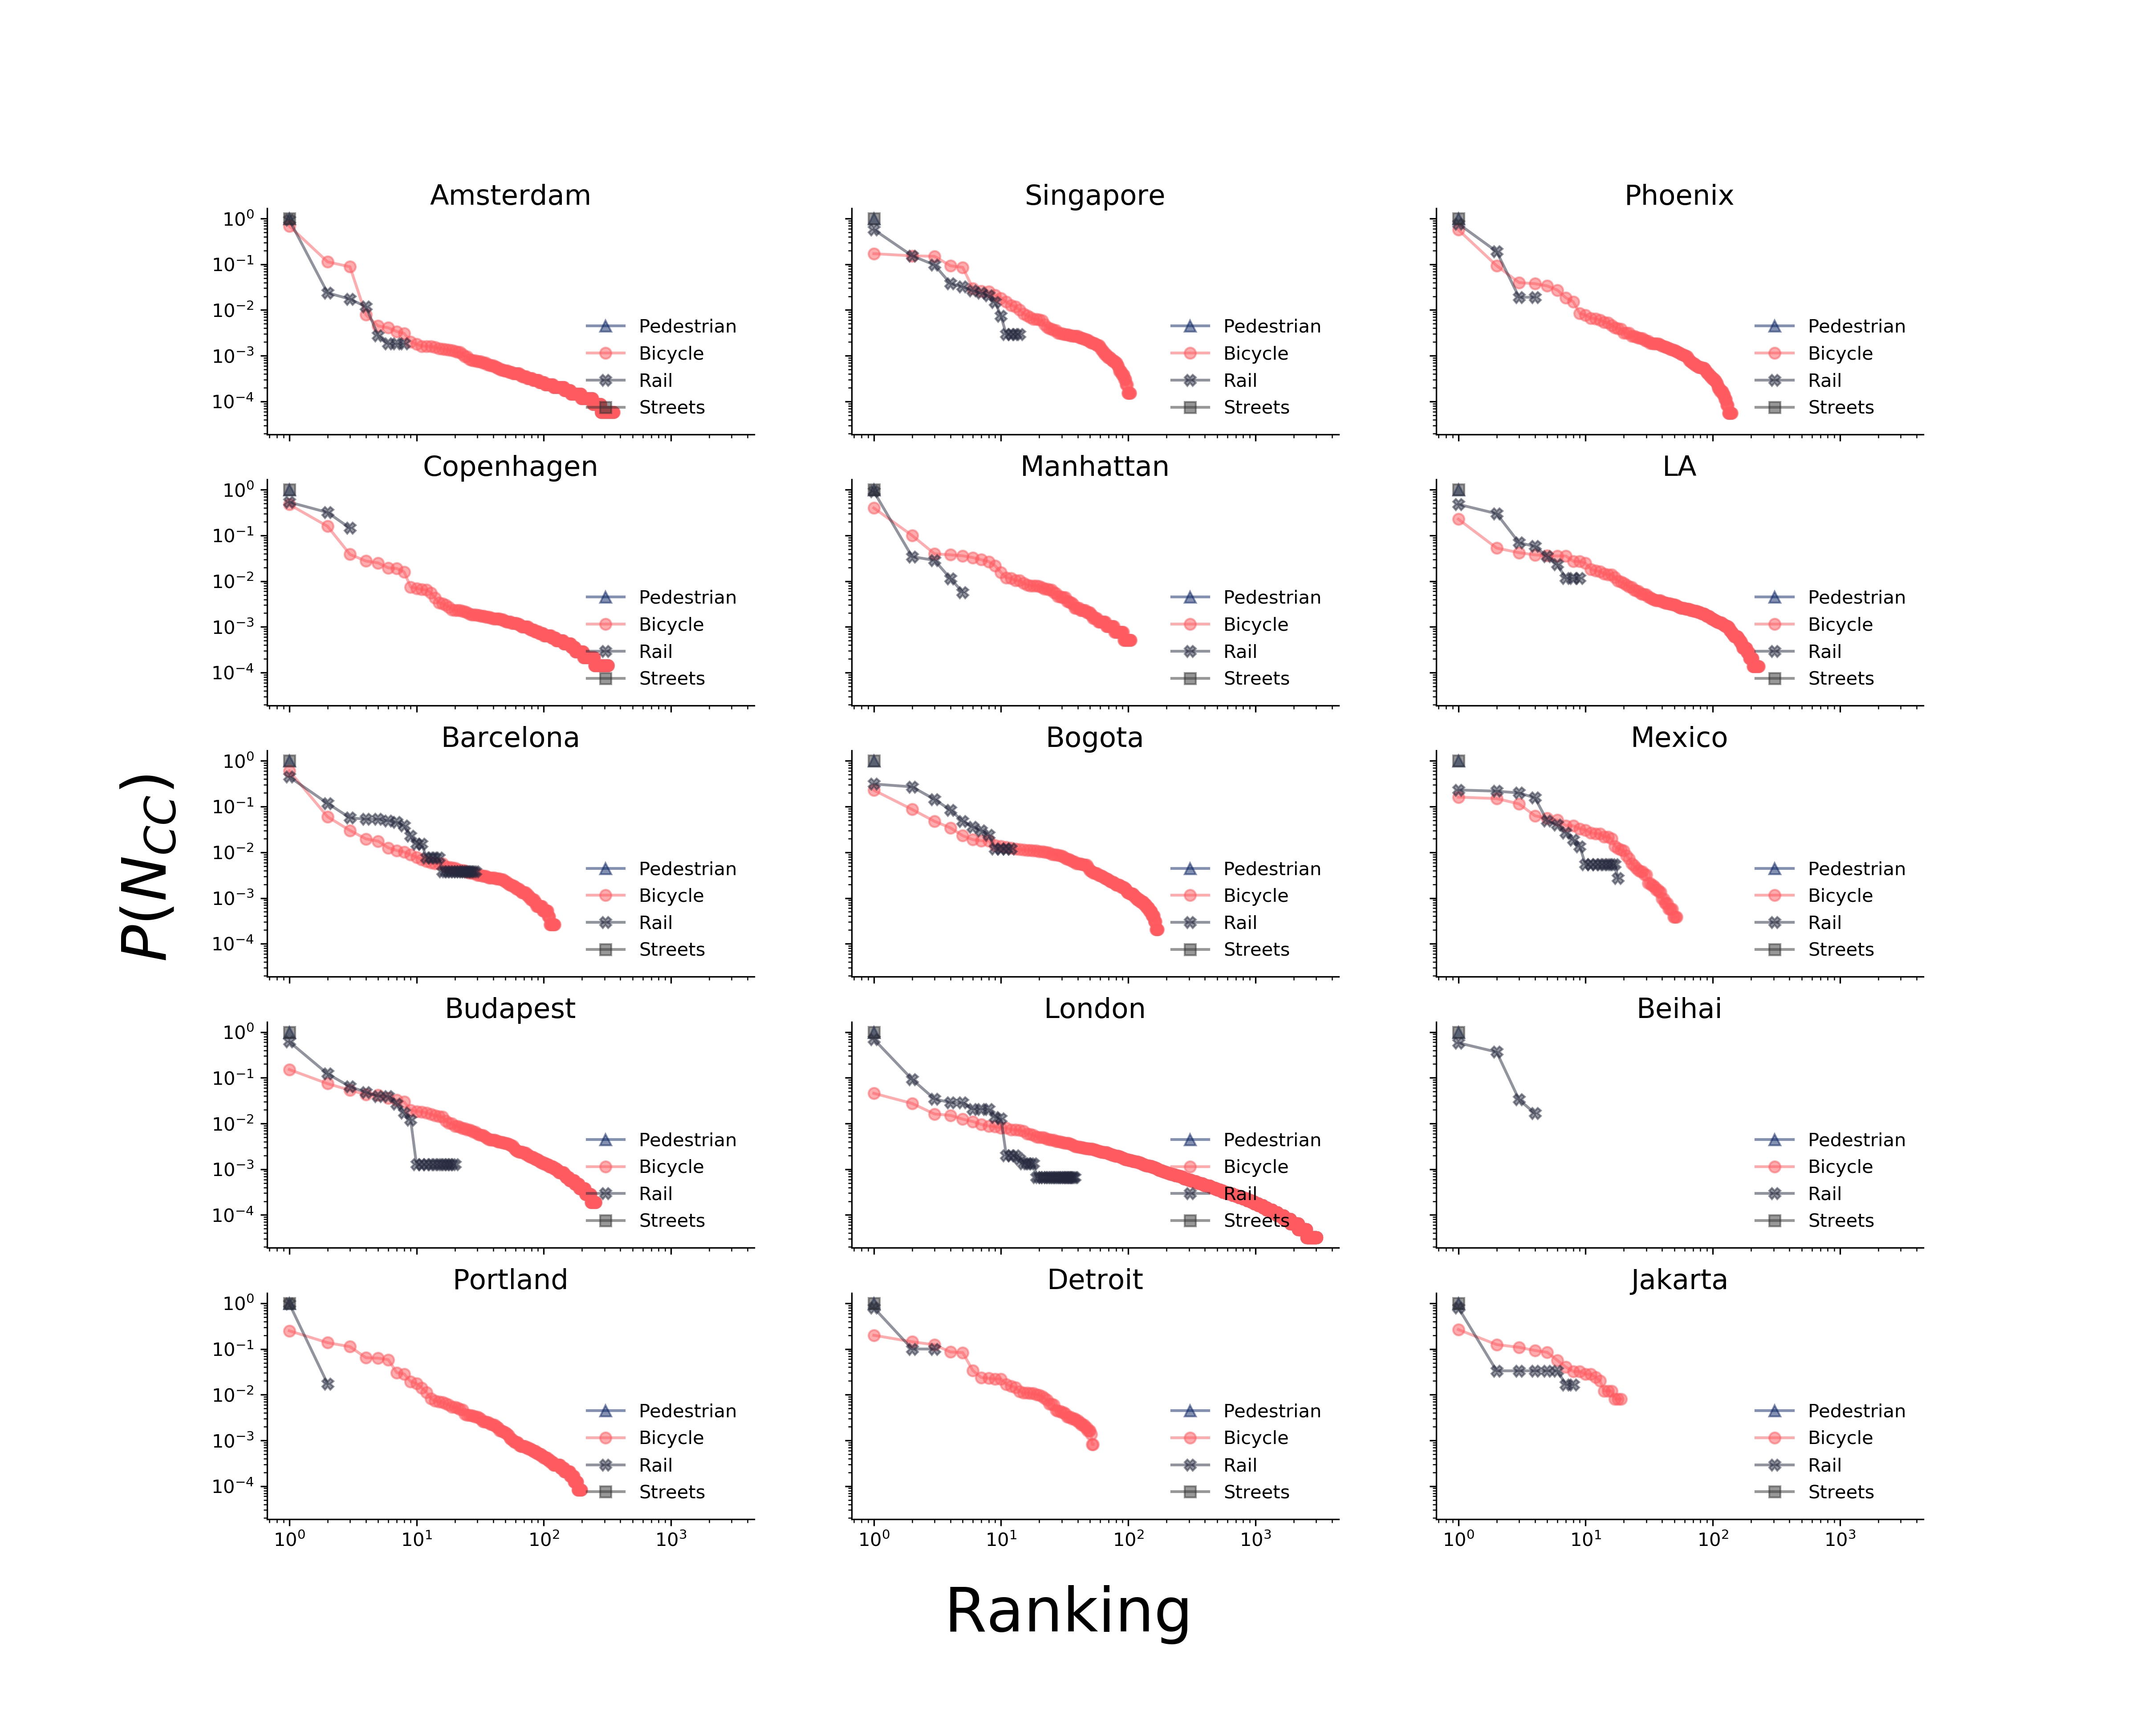
\includegraphics[width=0.8\textwidth]{images/datadriven/Nodes_cc.png}
  \caption[Connected component size distribution for analyzed cities]{The connected component size distribution [$P(N_{cc})$] for all cities and layers is well connected except in the bicycle layer. London has the most fragmented bicycle infrastructure layer, with more than 3000 components}
  \label{fig:Nodes}
\end{figure*}


% \subsection{Algorithms}
% We develop two main algorithms to improve the bicycle layer. The first algorithm, \textit{Largest-to-Second}, identifies in each step the largest connected component and connects it to the second largest. The second algorithm, \textit{Largest-to-Closest}, also identifies the largest connected component, but in each step connects it to the closest of the remaining components.

% To evaluate our algorithms we test them against a random baseline, \textit{Random-to-Closest}. In each step, \textit{Random-to-Closest} picks a component at random and connects it to the closest of the remaining components. We implement another baseline, the extreme case of \textit{Closest-Components}, which prioritizes connecting the closest two components.

% \begin{algorithm}[h!]
%   \caption{Largest-to-Second}\label{greedy_lcc}
%   \begin{algorithmic}[1]
%     \Procedure{\textit{L2S}}{}
%     \State $\textit{G} \gets \text{ bicycle network graph}$
%     \State $\textit{wcc} \gets \text{ components of network G}$
%     \For {i in length(wcc)-1}
%     \State  \text{sort \textit{wcc} by components size}
%     \State $\textit{cc} \gets \text{ two biggest components from \textit{wcc}}$
%     \State $\textit{i\_j} \gets \text{ closest nodes between } cc_0 \text{ and } cc_1$
%     \State $\text{connect } cc_0 \text{ and } cc_1 \text{ in } i\_j$
%     \EndFor
%     \EndProcedure
%   \end{algorithmic}
% \end{algorithm}

% \begin{algorithm}[h!]
%   \caption{Largest-to-Closest}\label{greedy_min}
%   \begin{algorithmic}[1]
%     \Procedure{\textit{L2C}}{}
%     \State $\textit{G} \gets \text{ bicycle network graph}$
%     \State $\textit{wcc} \gets \text{ components of network G}$
%     \For {i in length(wcc)-1}
%     \State  \text{sort \textit{wcc} by components size}
%     \State $cc_0 \gets \text{ biggest component from \textit{wcc}}$
%     \State $cc_n \gets \text{ clossest component to } cc_0$
%     \State $\textit{i\_j} \gets \text{ closest nodes between } cc_0 \text{ and } cc_n$
%     \State $\text{connect } cc_0 \text{ and } cc_n \text{ in } i\_j$
%     \EndFor
%     \EndProcedure
%   \end{algorithmic}
% \end{algorithm}

% \begin{algorithm}[h!]
%   \caption{Random-to-Closest}\label{random}
%   \begin{algorithmic}[1]
%     \Procedure{\textit{R2C}}{}
%     \State $\textit{G} \gets \text{ bicycle network graph}$
%     \State $\textit{wcc} \gets \text{ components of network G}$
%     \For {i in length(wcc)-1}
%     \State $cc_{ran} \gets \text{ random component from \textit{wcc}}$
%     \State $cc_n \gets \text{ clossest component to } cc_{ran}$
%     \State $\textit{i\_j} \gets \text{ closest nodes between } cc_{ran} \text{ and } cc_n$
%     \State $\text{connect } cc_{ran} \text{ and } cc_n \text{ in } i\_j$
%     \EndFor
%     \EndProcedure
%   \end{algorithmic}
% \end{algorithm}

% \begin{algorithm}[h!]
%   \caption{Closest-Components}\label{min_delta}
%   \begin{algorithmic}[1]
%     \Procedure{\textit{CC}}{}
%     \State $\textit{G} \gets \text{ bicycle network graph}$
%     \State $\textit{wcc} \gets \text{ components of network G}$
%     \For {i in length(wcc)-1}
%     \State $\Delta_{min} \gets \text{ clossest components in \textit{wcc}}$
%     \State $cc_{0} \gets \text{ first component for }\Delta_{min}$
%     \State $cc_{1} \gets \text{ second component for } \Delta_{min}$
%     \State $\textit{i\_j} \gets \text{ closest nodes between } cc_{0} \text{ and } cc_{1}$
%     \State $\text{connect } cc_{0} \text{ and } cc_{1} \text{ in } i\_j$
%     \EndFor
%     \EndProcedure
%   \end{algorithmic}
% \end{algorithm}

\subsection{Bicycle network improvement}\label{SI:BikeImprovement}

Here we show the improvement of the bicycle network after the implementation of the algorithms. We measure the improvement with four different metrics. Two of them implement the notion of connectedness: i) Fraction of nodes inside the largest connected component compared to the total number of nodes in the bicycle layer, and ii) the fraction of link kilometers inside the largest connected component. In Figure \ref{fig:NodesIncrease} and \ref{fig:Lengthsncrease} we show these two measures for fourteen different cities. We also quantify iii) bicycle-to-car directness to answer the question ``how direct are the average routes of bicycles compared to cars?''. Finally, in order to measure the cumulative efficiency of our algorithms, we define the metric: iv) $G_{LCC}$ as the relative gain of bicycle path kilometers in the largest connected component. In Figures \ref{fig:Directness} and \ref{fig:Gain} we report these two measures for all algorithms and cities considered.

\begin{figure*}[h!]
  \centering
  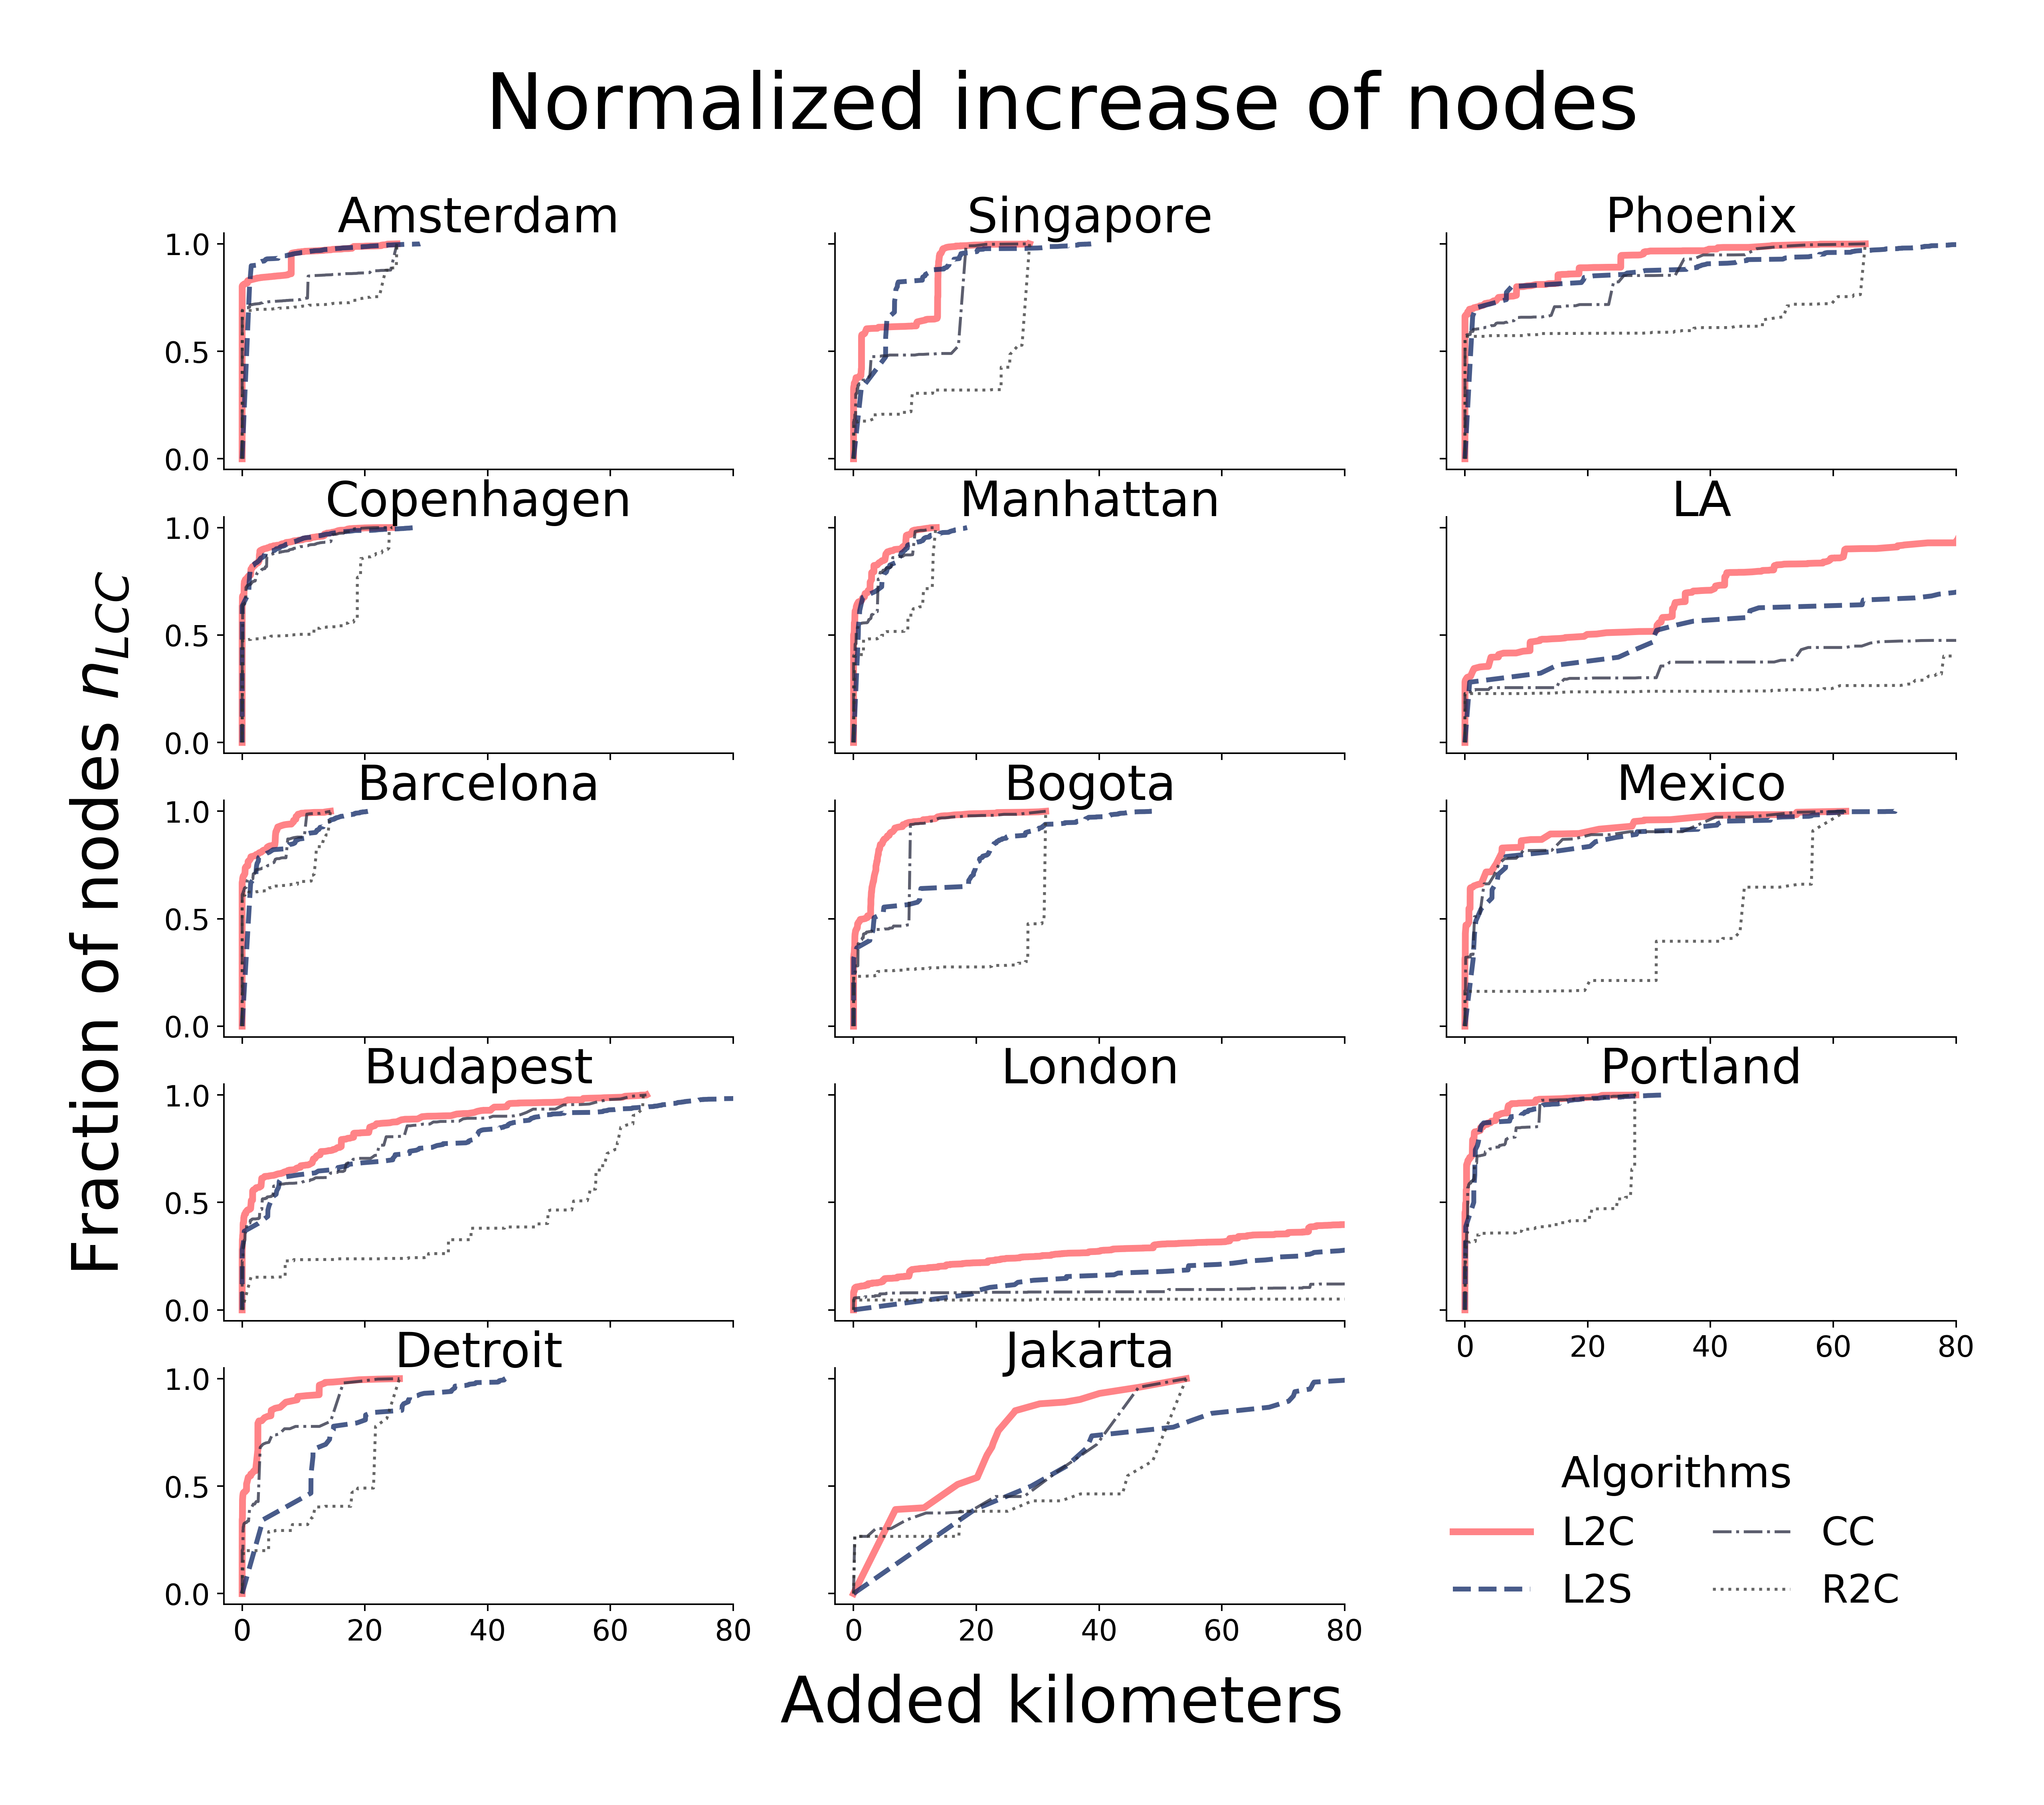
\includegraphics[width=0.8\textwidth]{images/datadriven/SI_Nodes.png}
  \caption{Normalized increase in nodes inside the largest connected component ($n_{LCC}$).}
  \label{fig:NodesIncrease}
\end{figure*}

\begin{figure*}[h!]
  \centering
  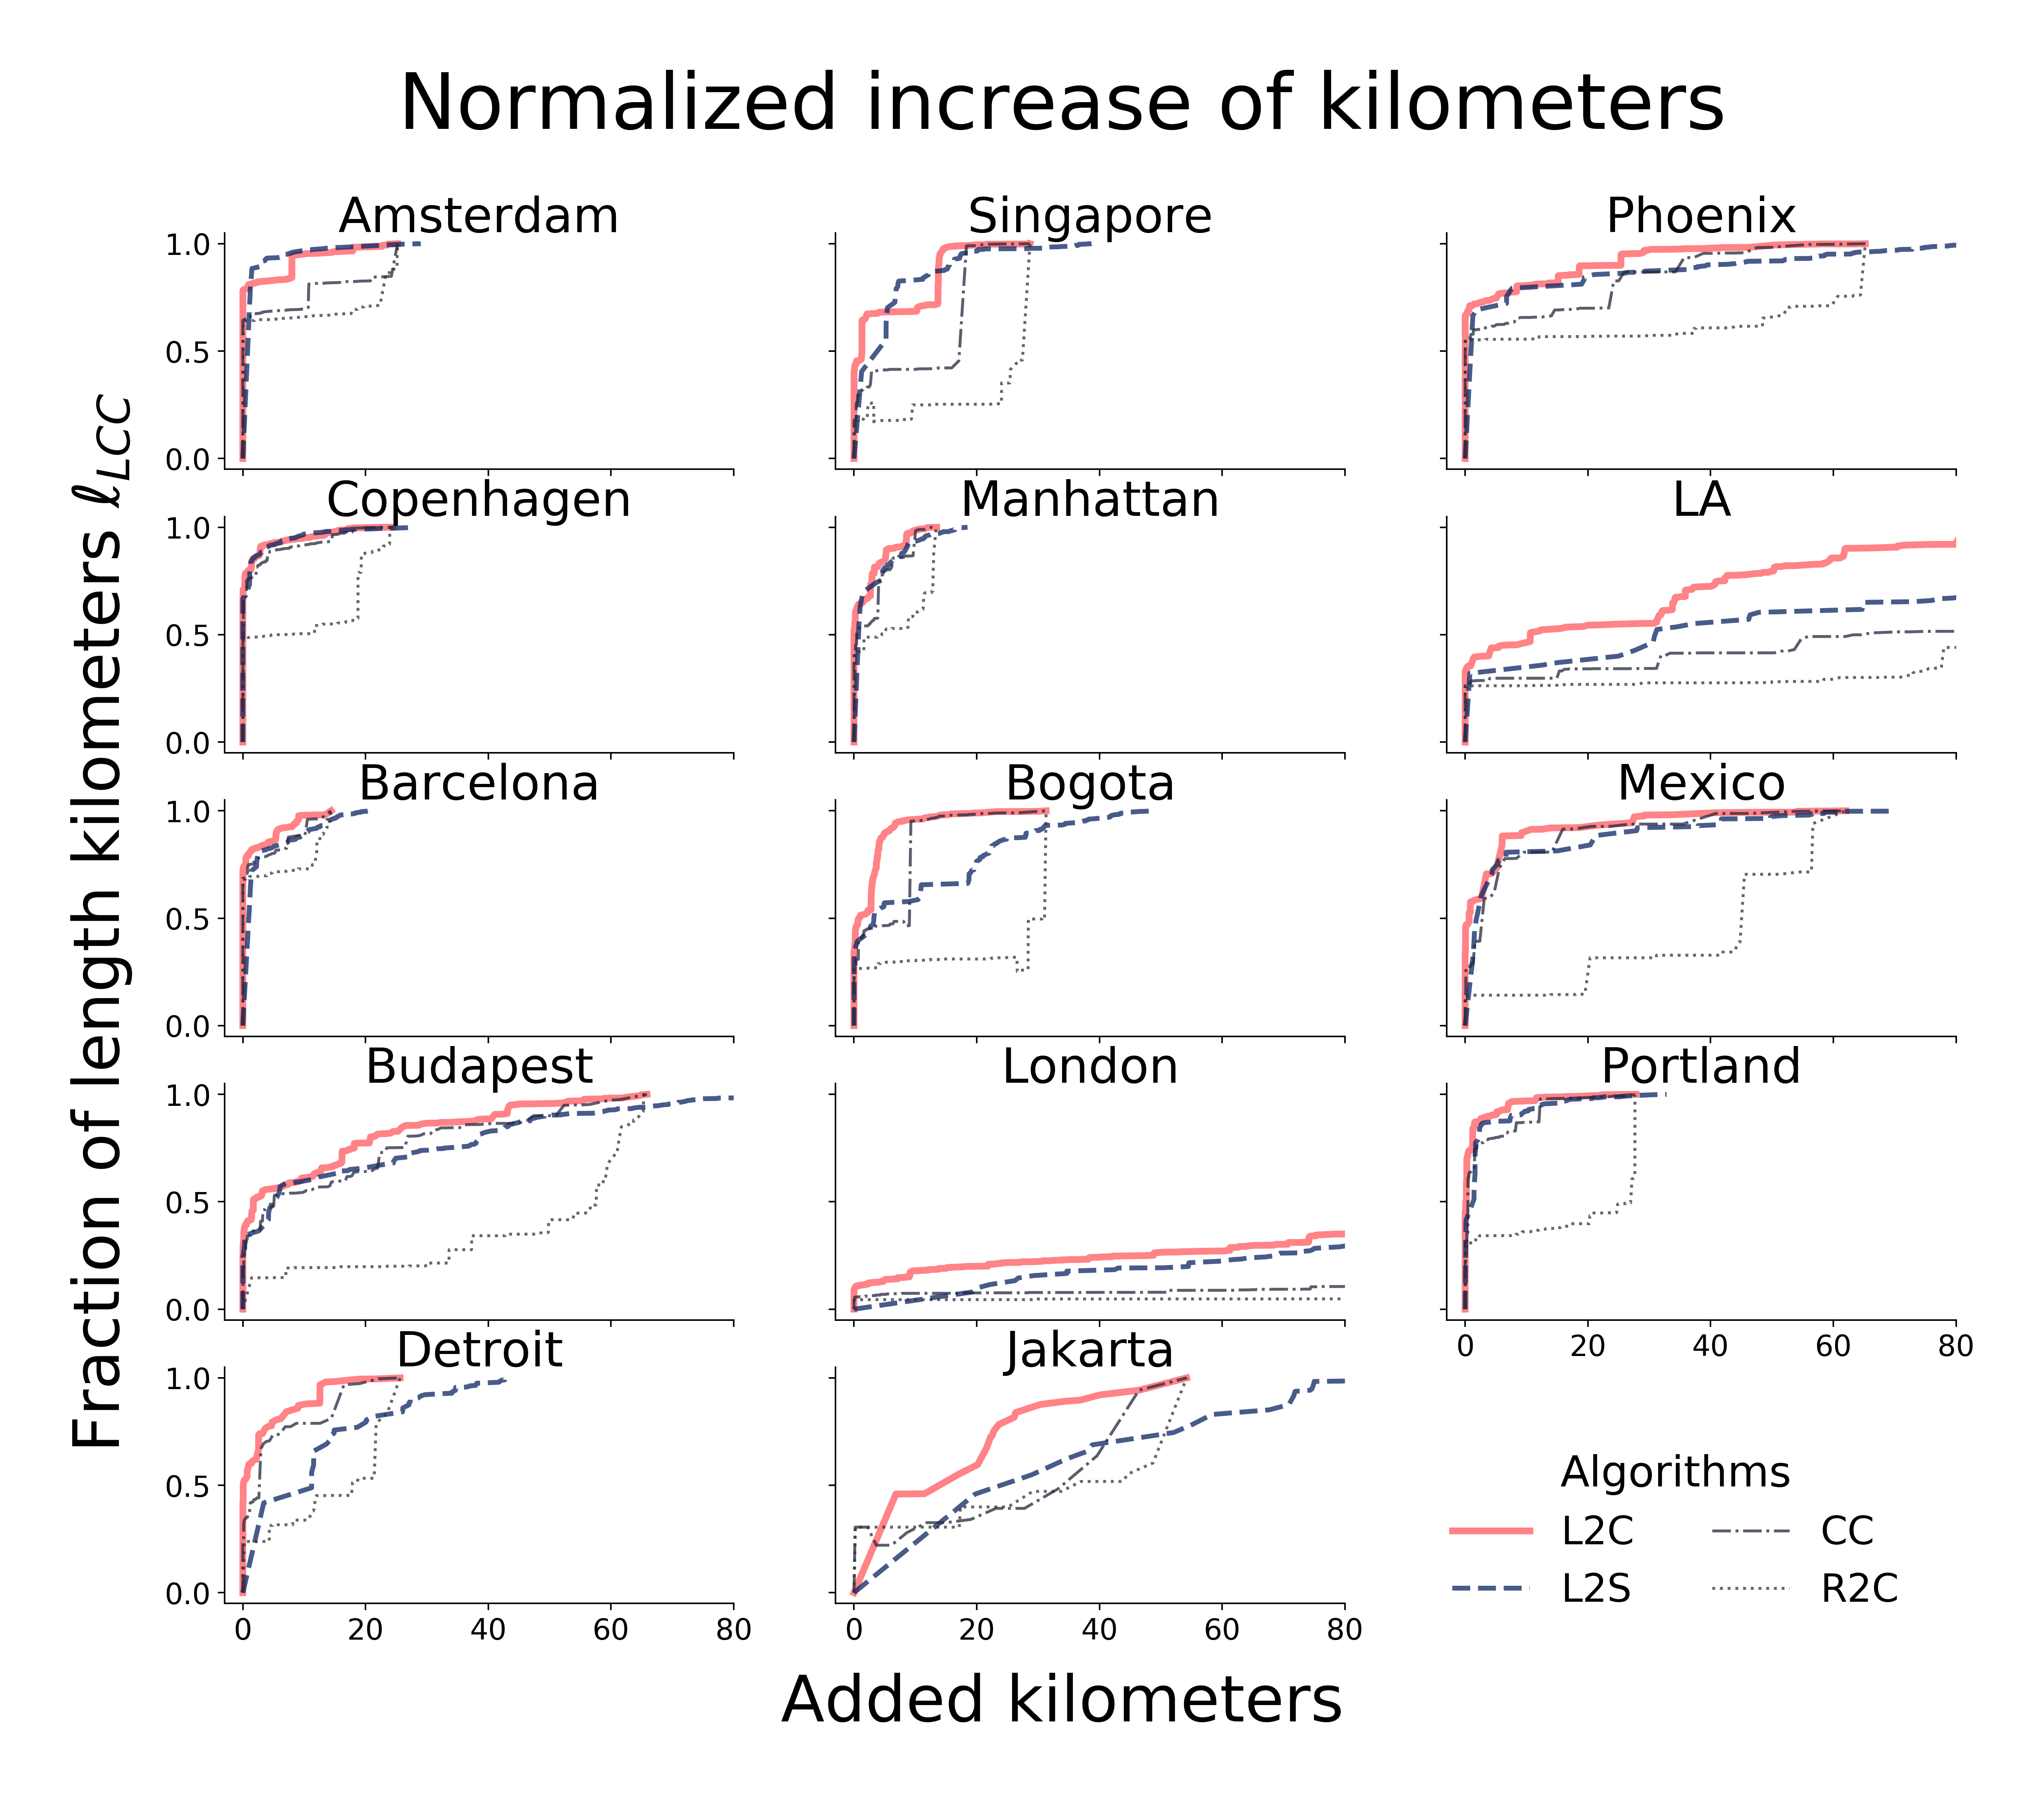
\includegraphics[width=0.8\textwidth]{images/datadriven/SI_Lengths.png}
  \caption{Normalized increase in kilometers inside the largest connected component ($\ell_{LCC}$).}
  \label{fig:LengthsIncrease}
\end{figure*}

\begin{figure*}[h!]
  \centering
  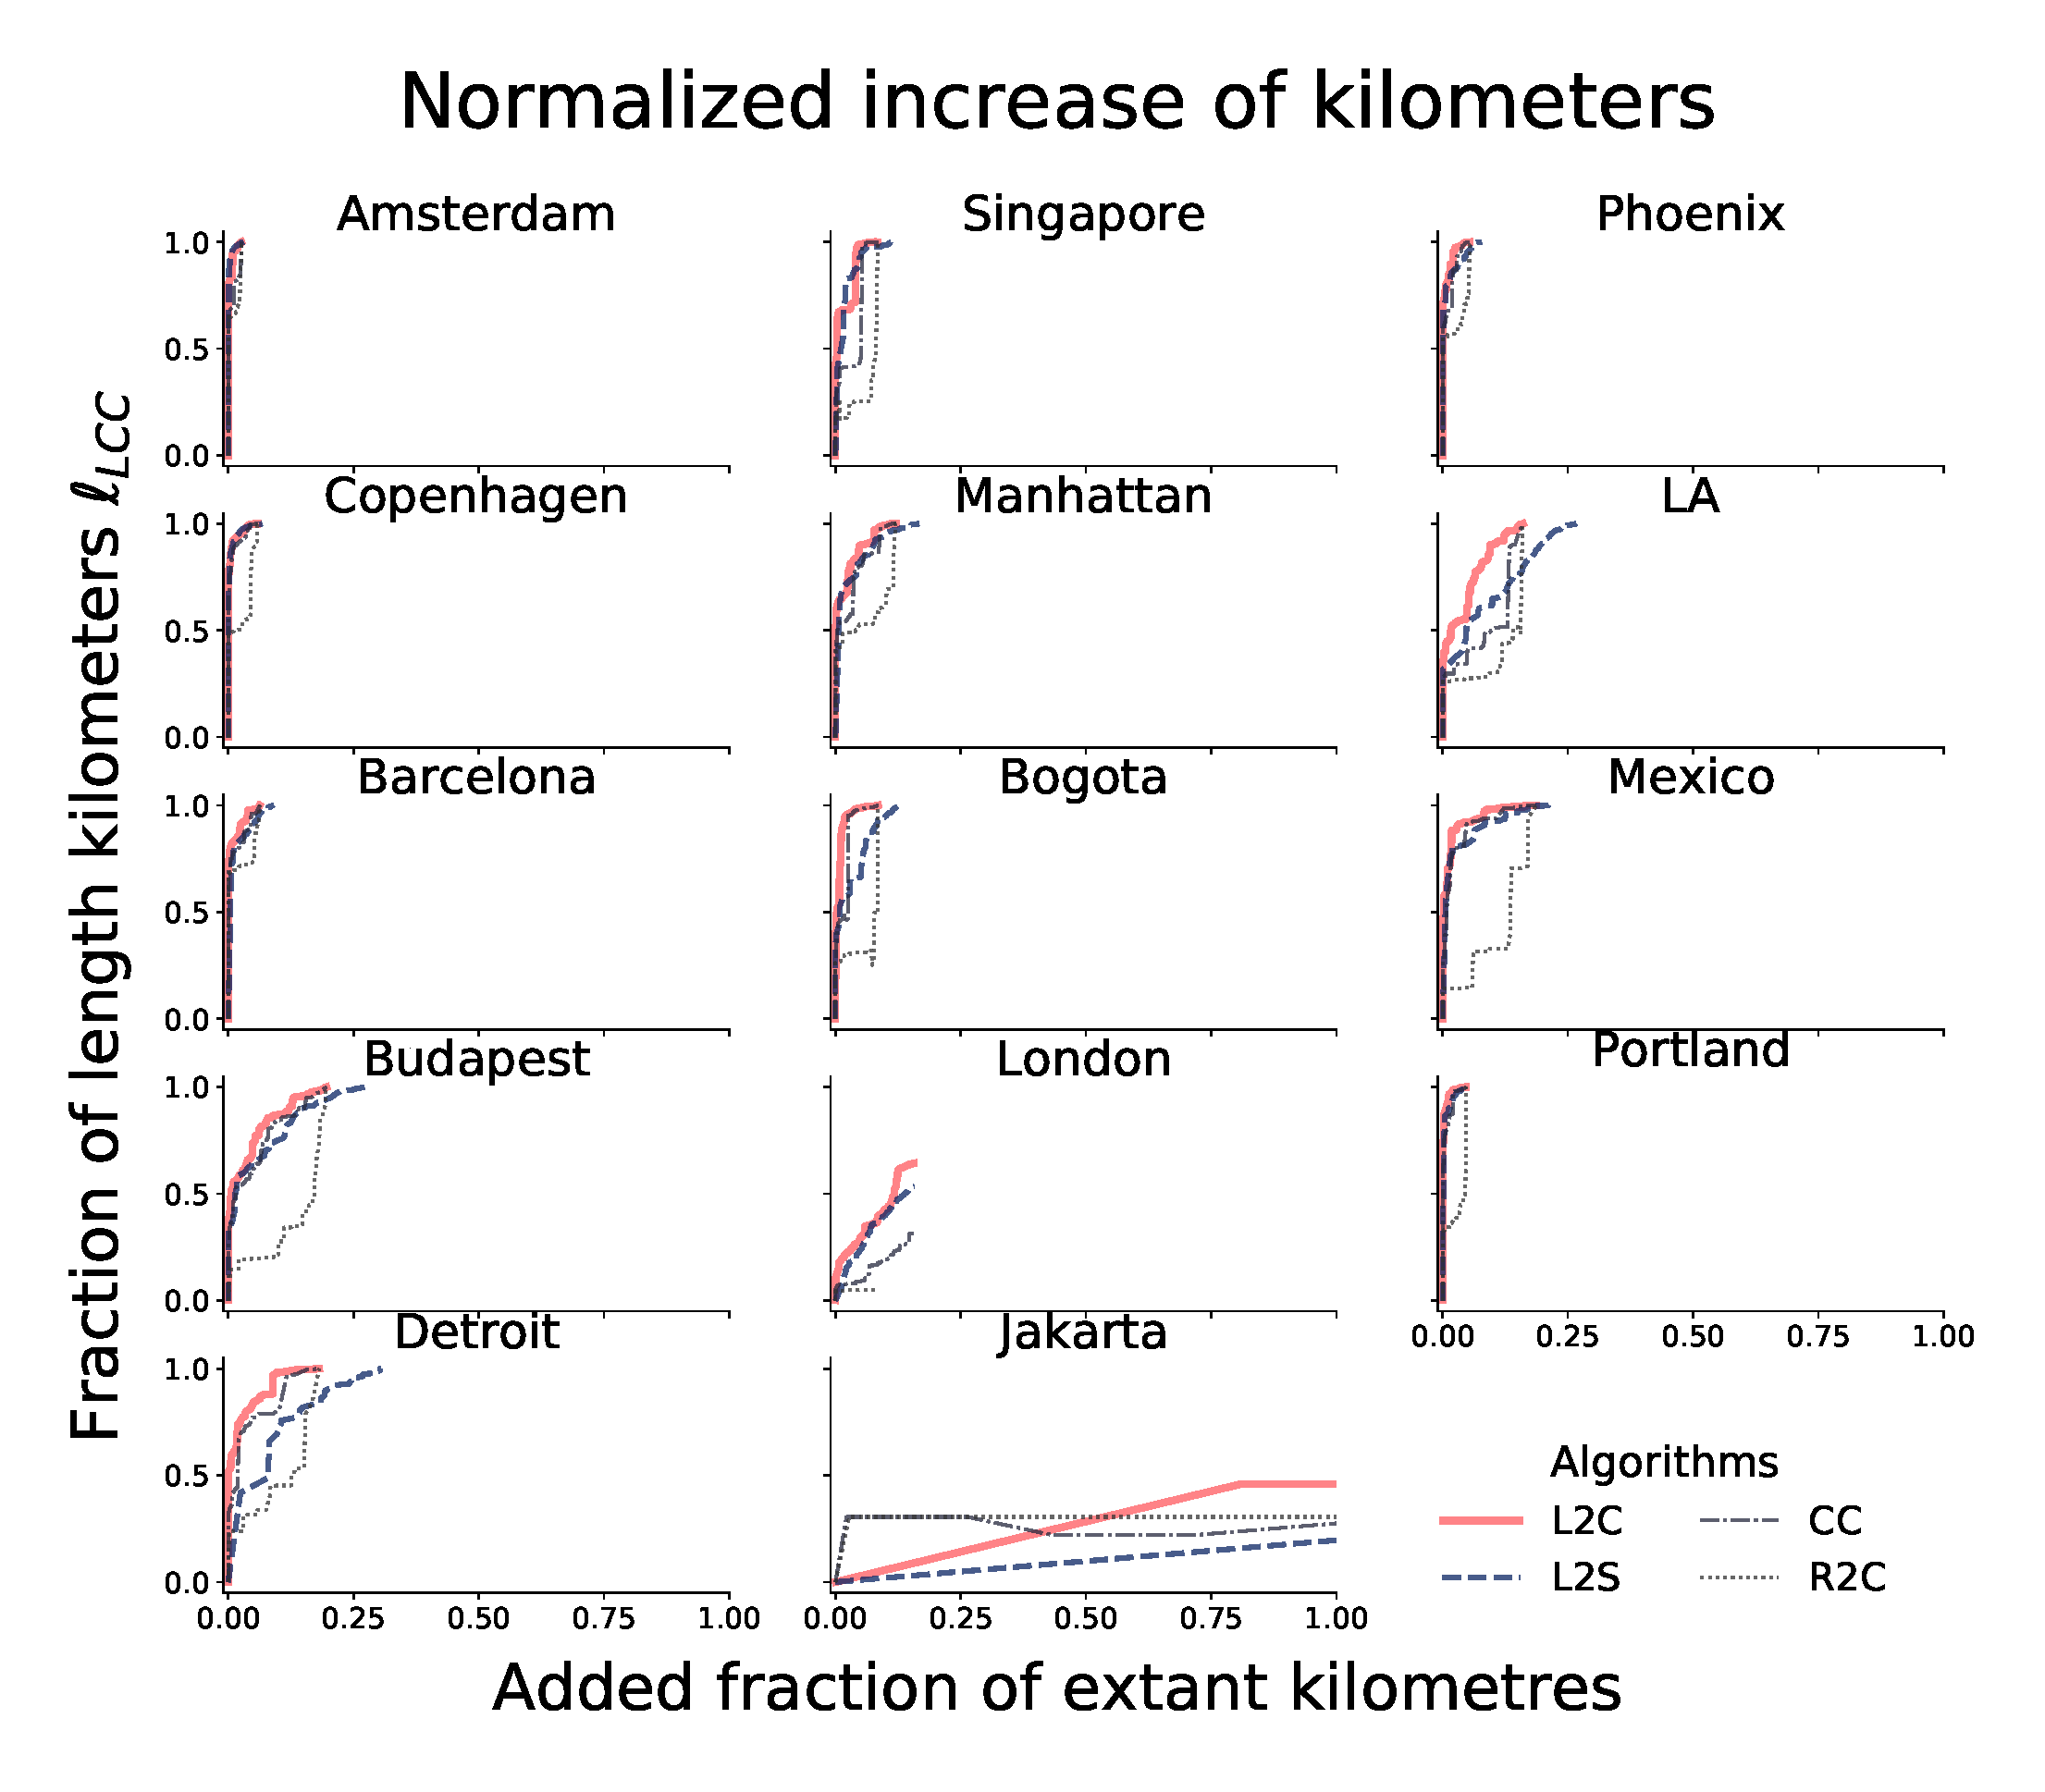
\includegraphics[width=0.8\textwidth]{images/datadriven/SI_Lengths_Bike-Streets_FractionKM.pdf}
  \caption{Normalized increase in kilometers inside the largest connected component ($\ell_{LCC}$) versus the fraction of extant kilometers to be added.}
  \label{fig:Lengthsncrease_norm}
\end{figure*}

\begin{figure*}[h!]
  \centering
  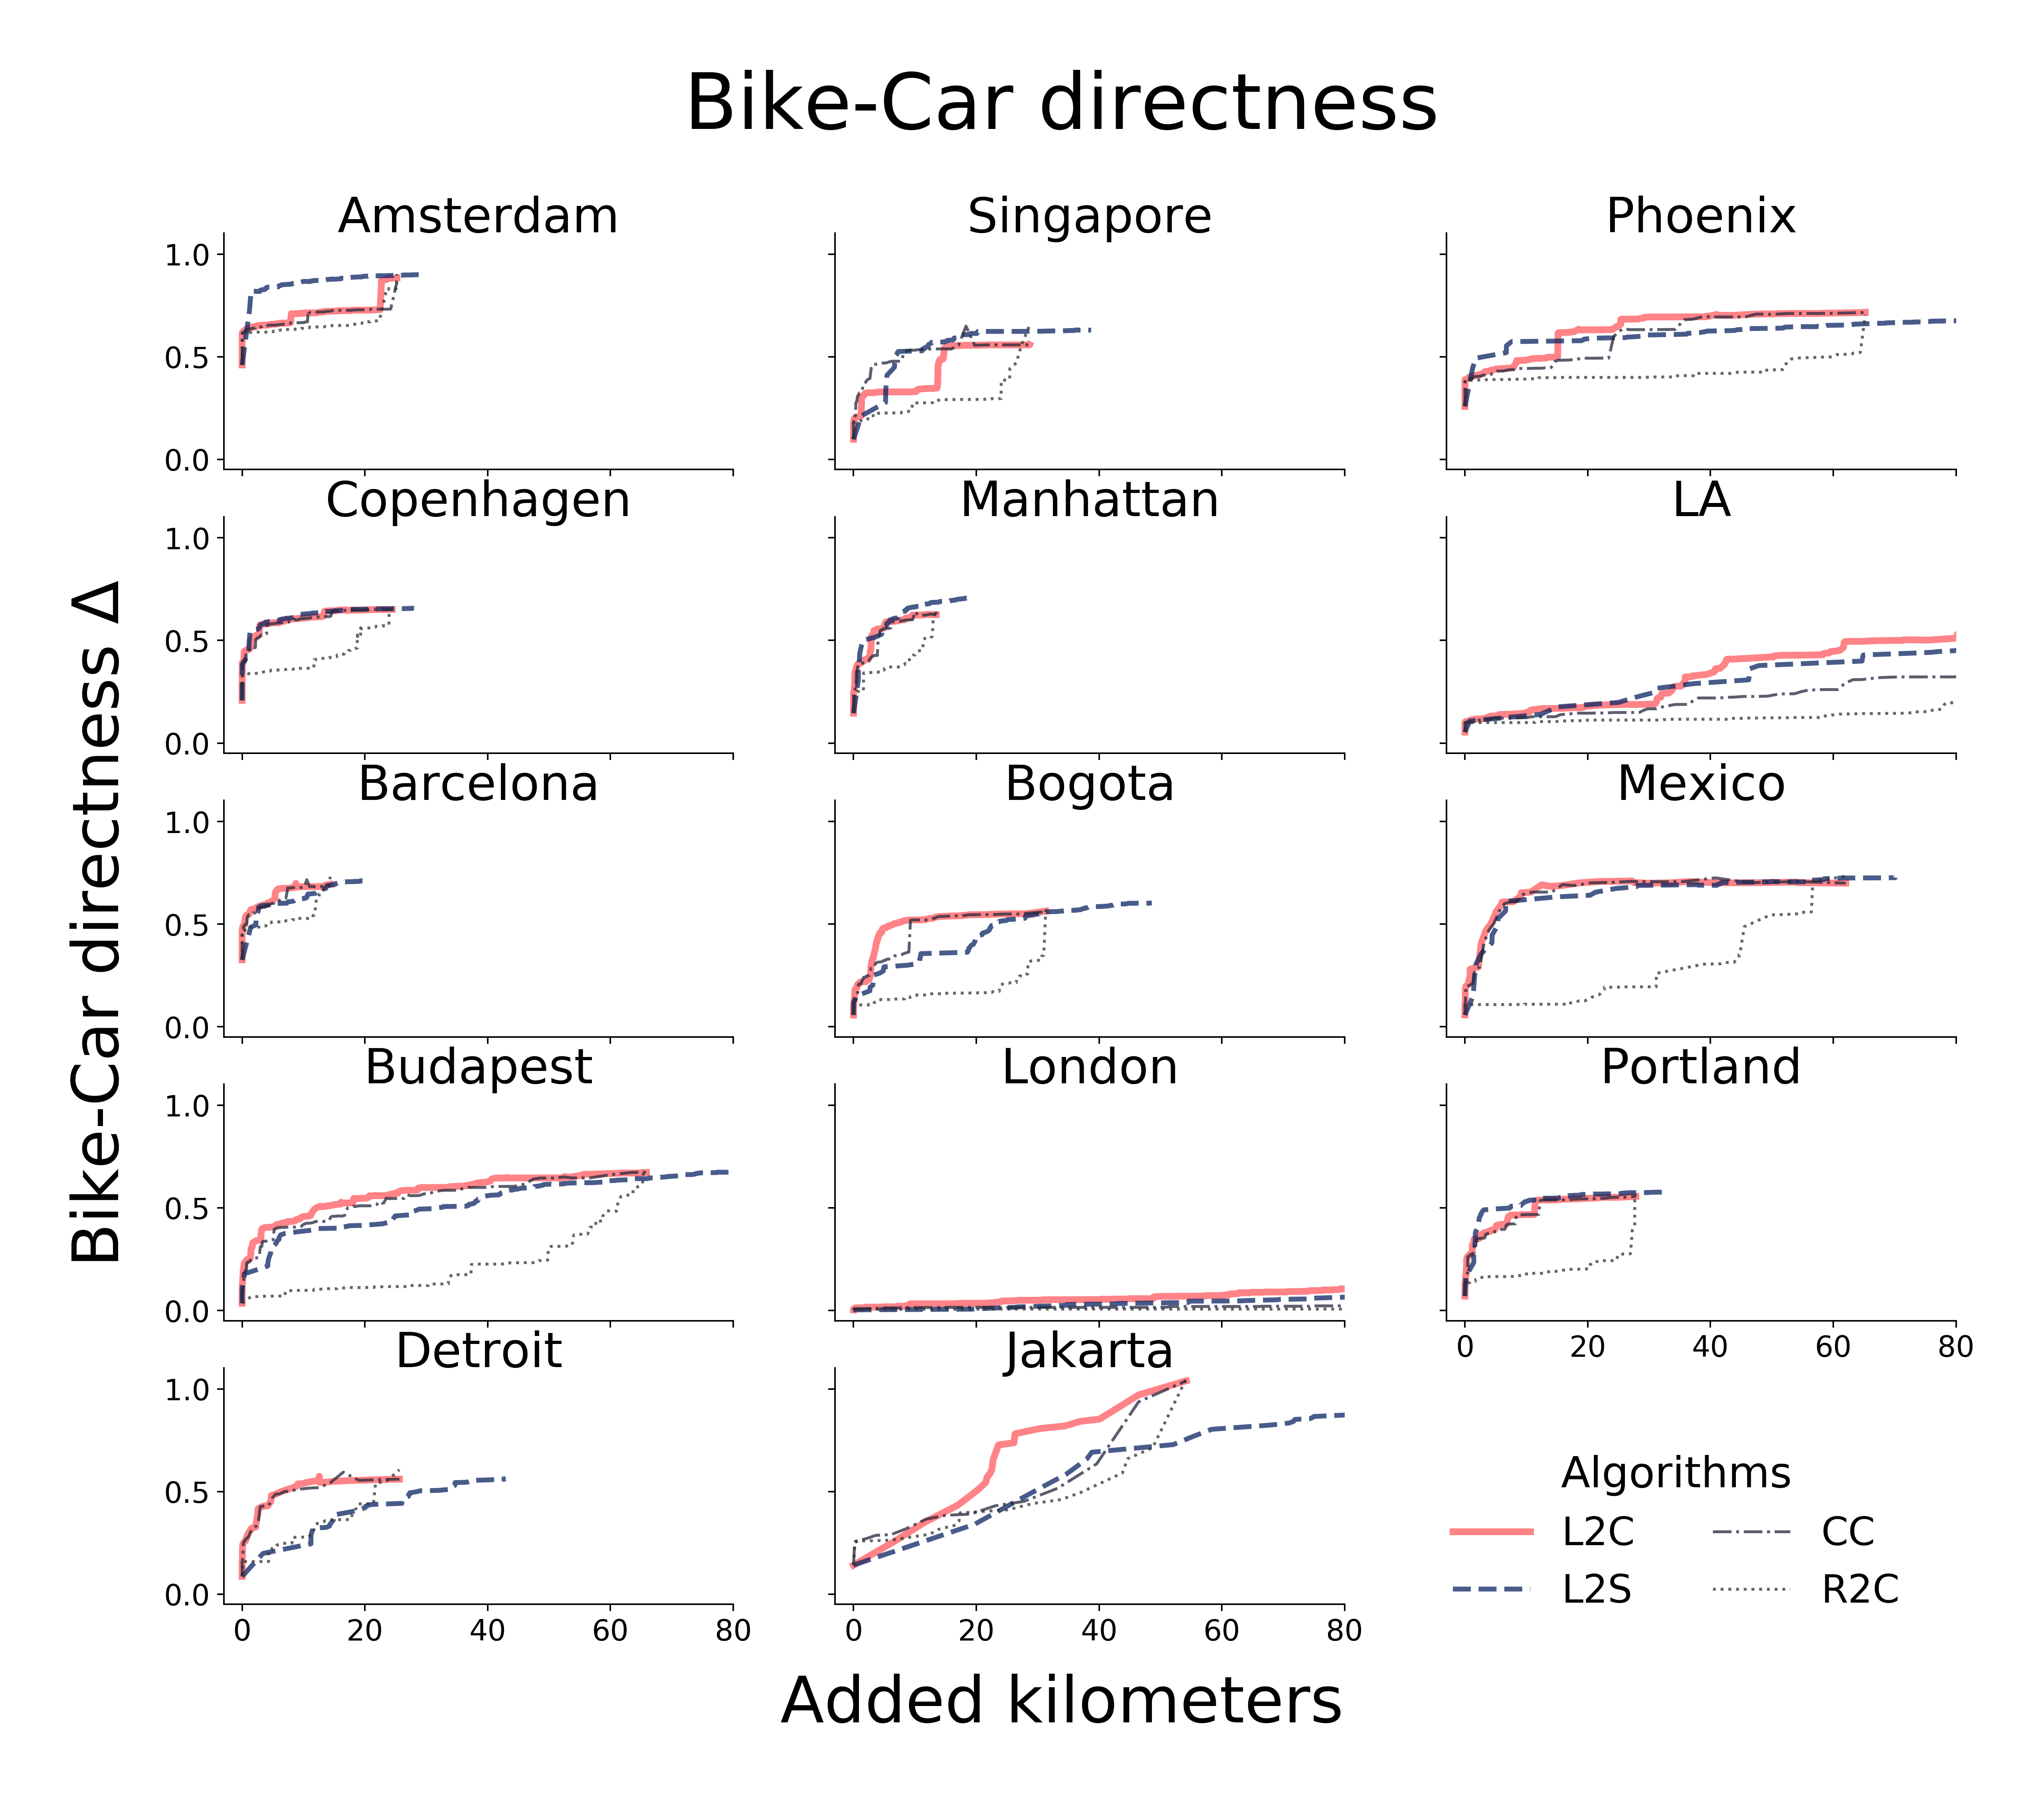
\includegraphics[width=0.8\textwidth]{images/datadriven/SI_Directness.png}
  \caption{Bike-car directness $\Delta$ per invested kilometers.}
  \label{fig:Directness}
\end{figure*}

\begin{figure*}[h!]
  \centering
  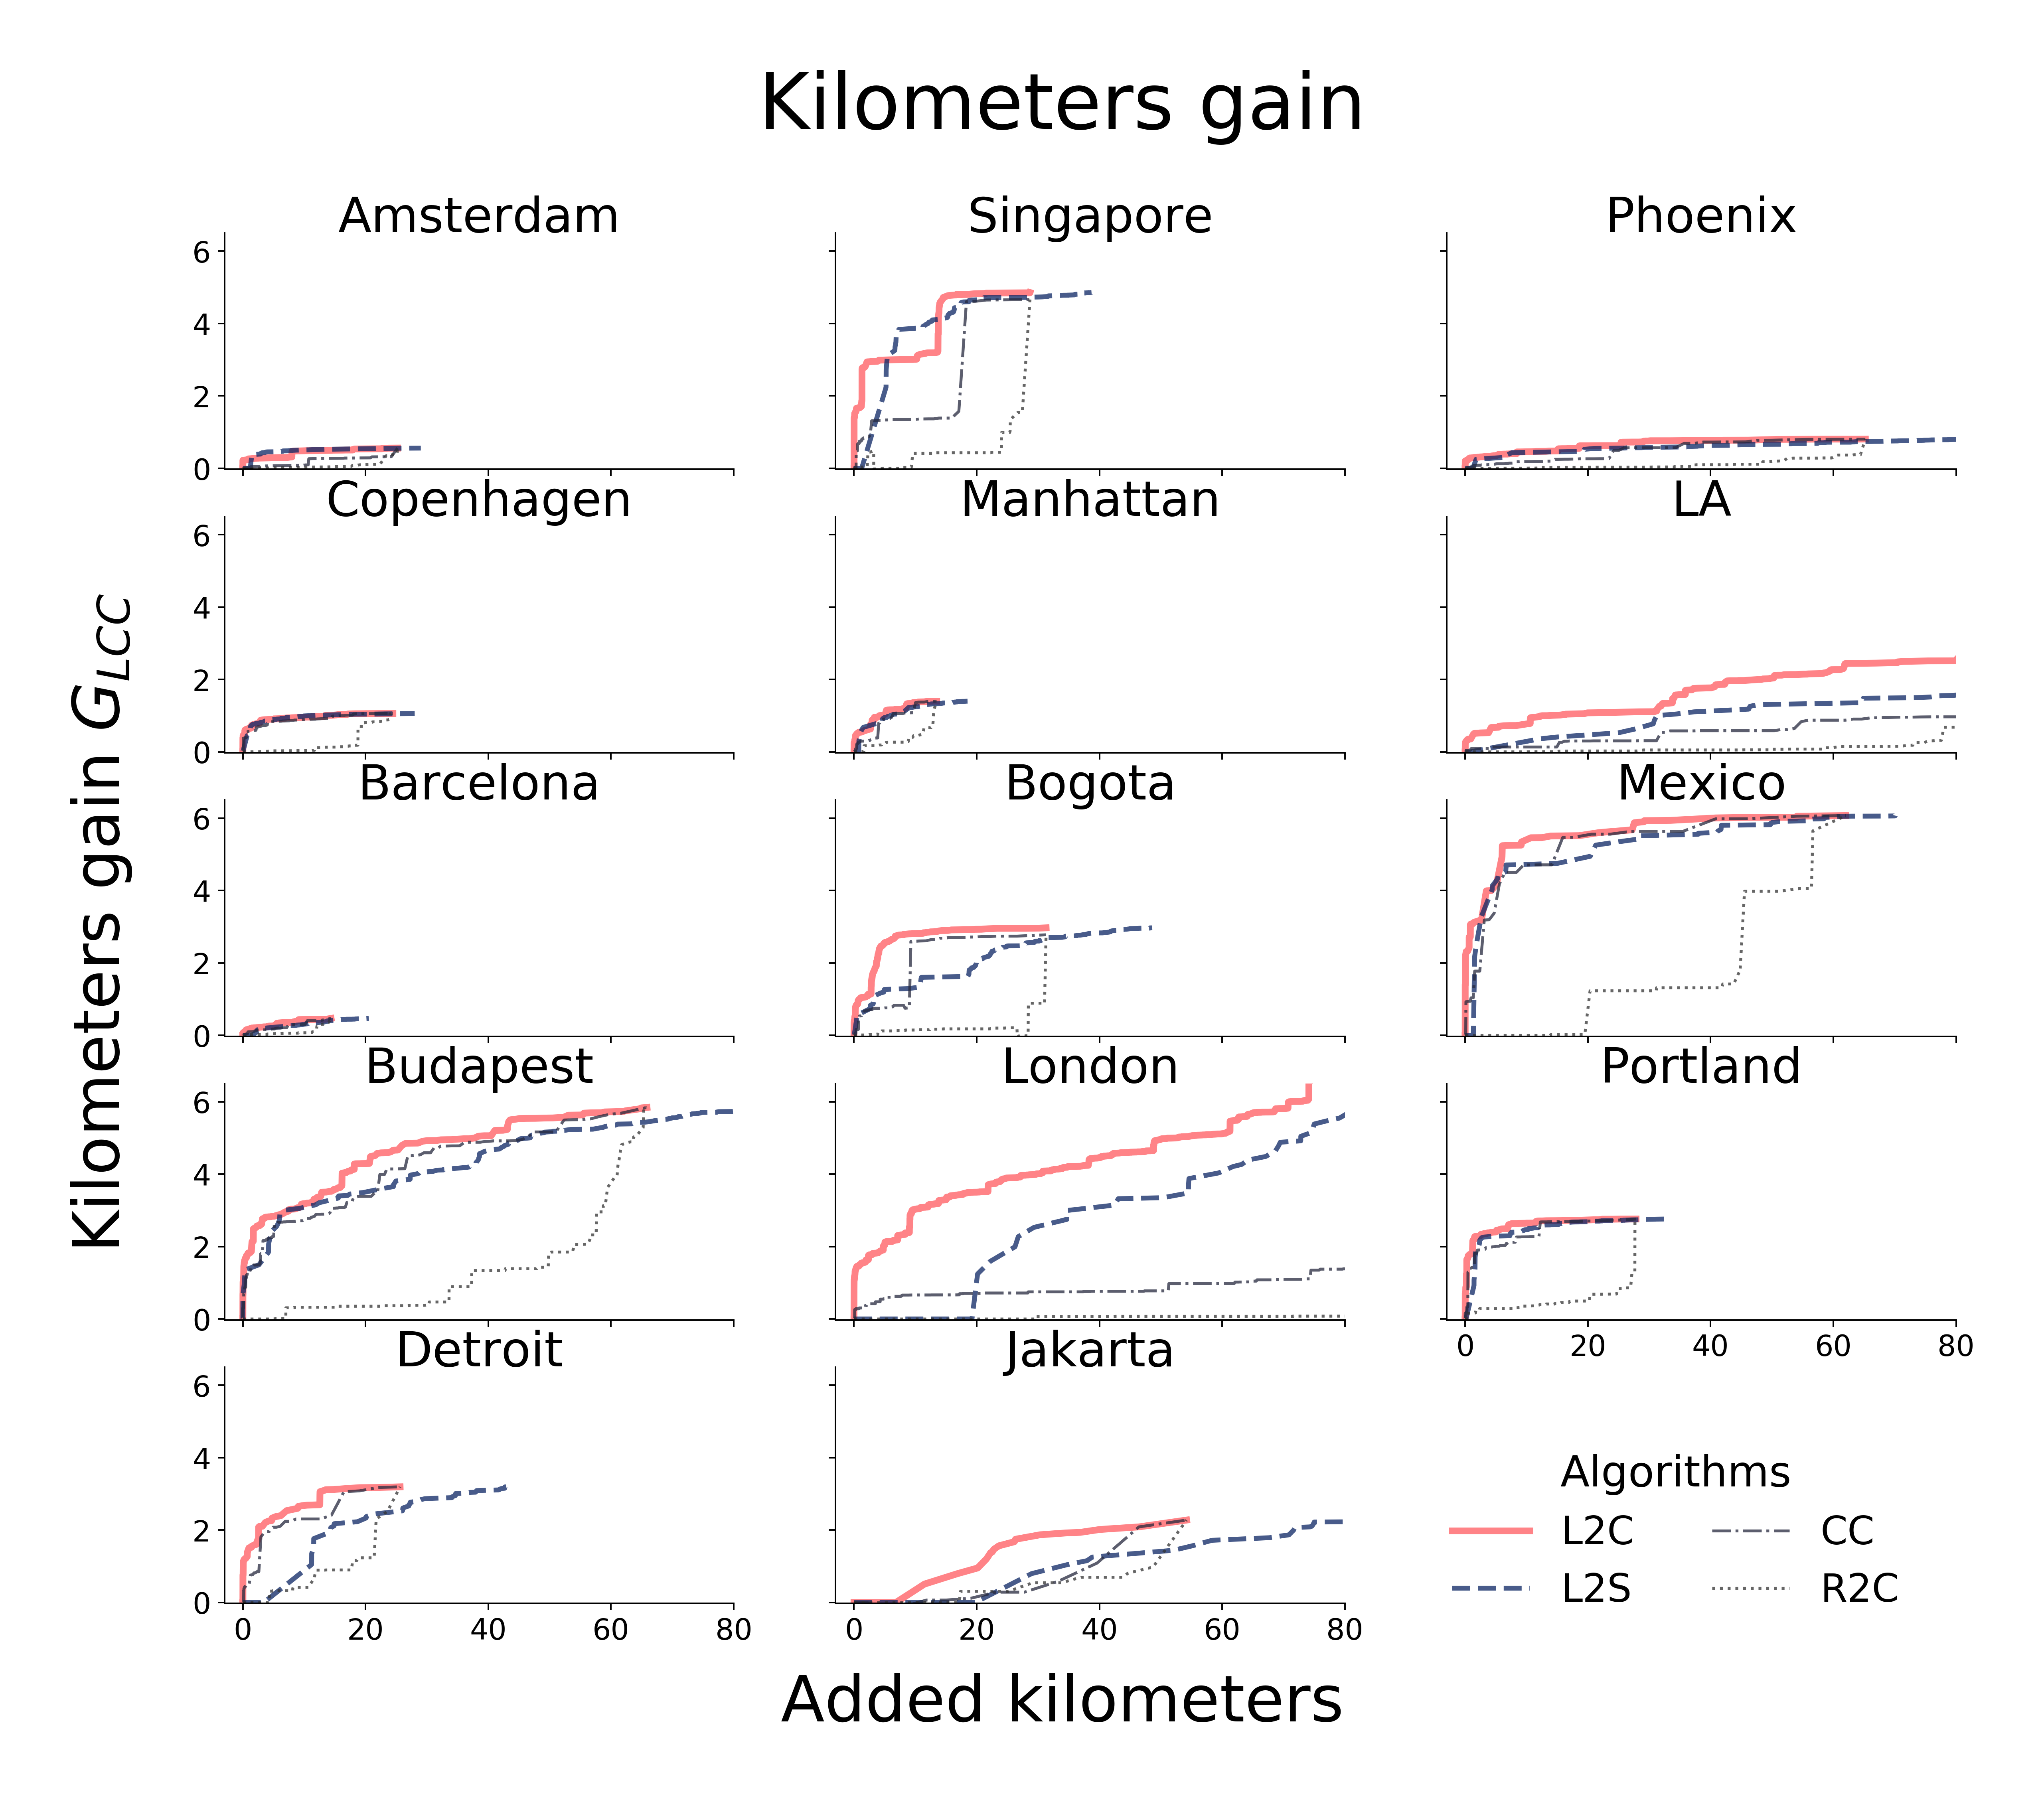
\includegraphics[width=0.8\textwidth]{images/datadriven/SI_Gain.png}
  \caption{Kilometers gain in the largest connected component.}
  \label{fig:Gain}
\end{figure*}


\subsection{Bicycle network and 30 km/hr streets}\label{SI:BikeStreets}
We applied the algorithms to the bicycle infrastructure and all the bikeable streets, those with a speed limit of $30\ km/hr$ or less (see Figures~\ref{fig:NodesIncrease_BikeStreets}, \ref{fig:Lengthsncrease_BikeStreets}, \ref{fig:Directness_BikeStreets}, and \ref{fig:Gain_BikeStreets}).

\begin{figure*}[h!]
  \centering
  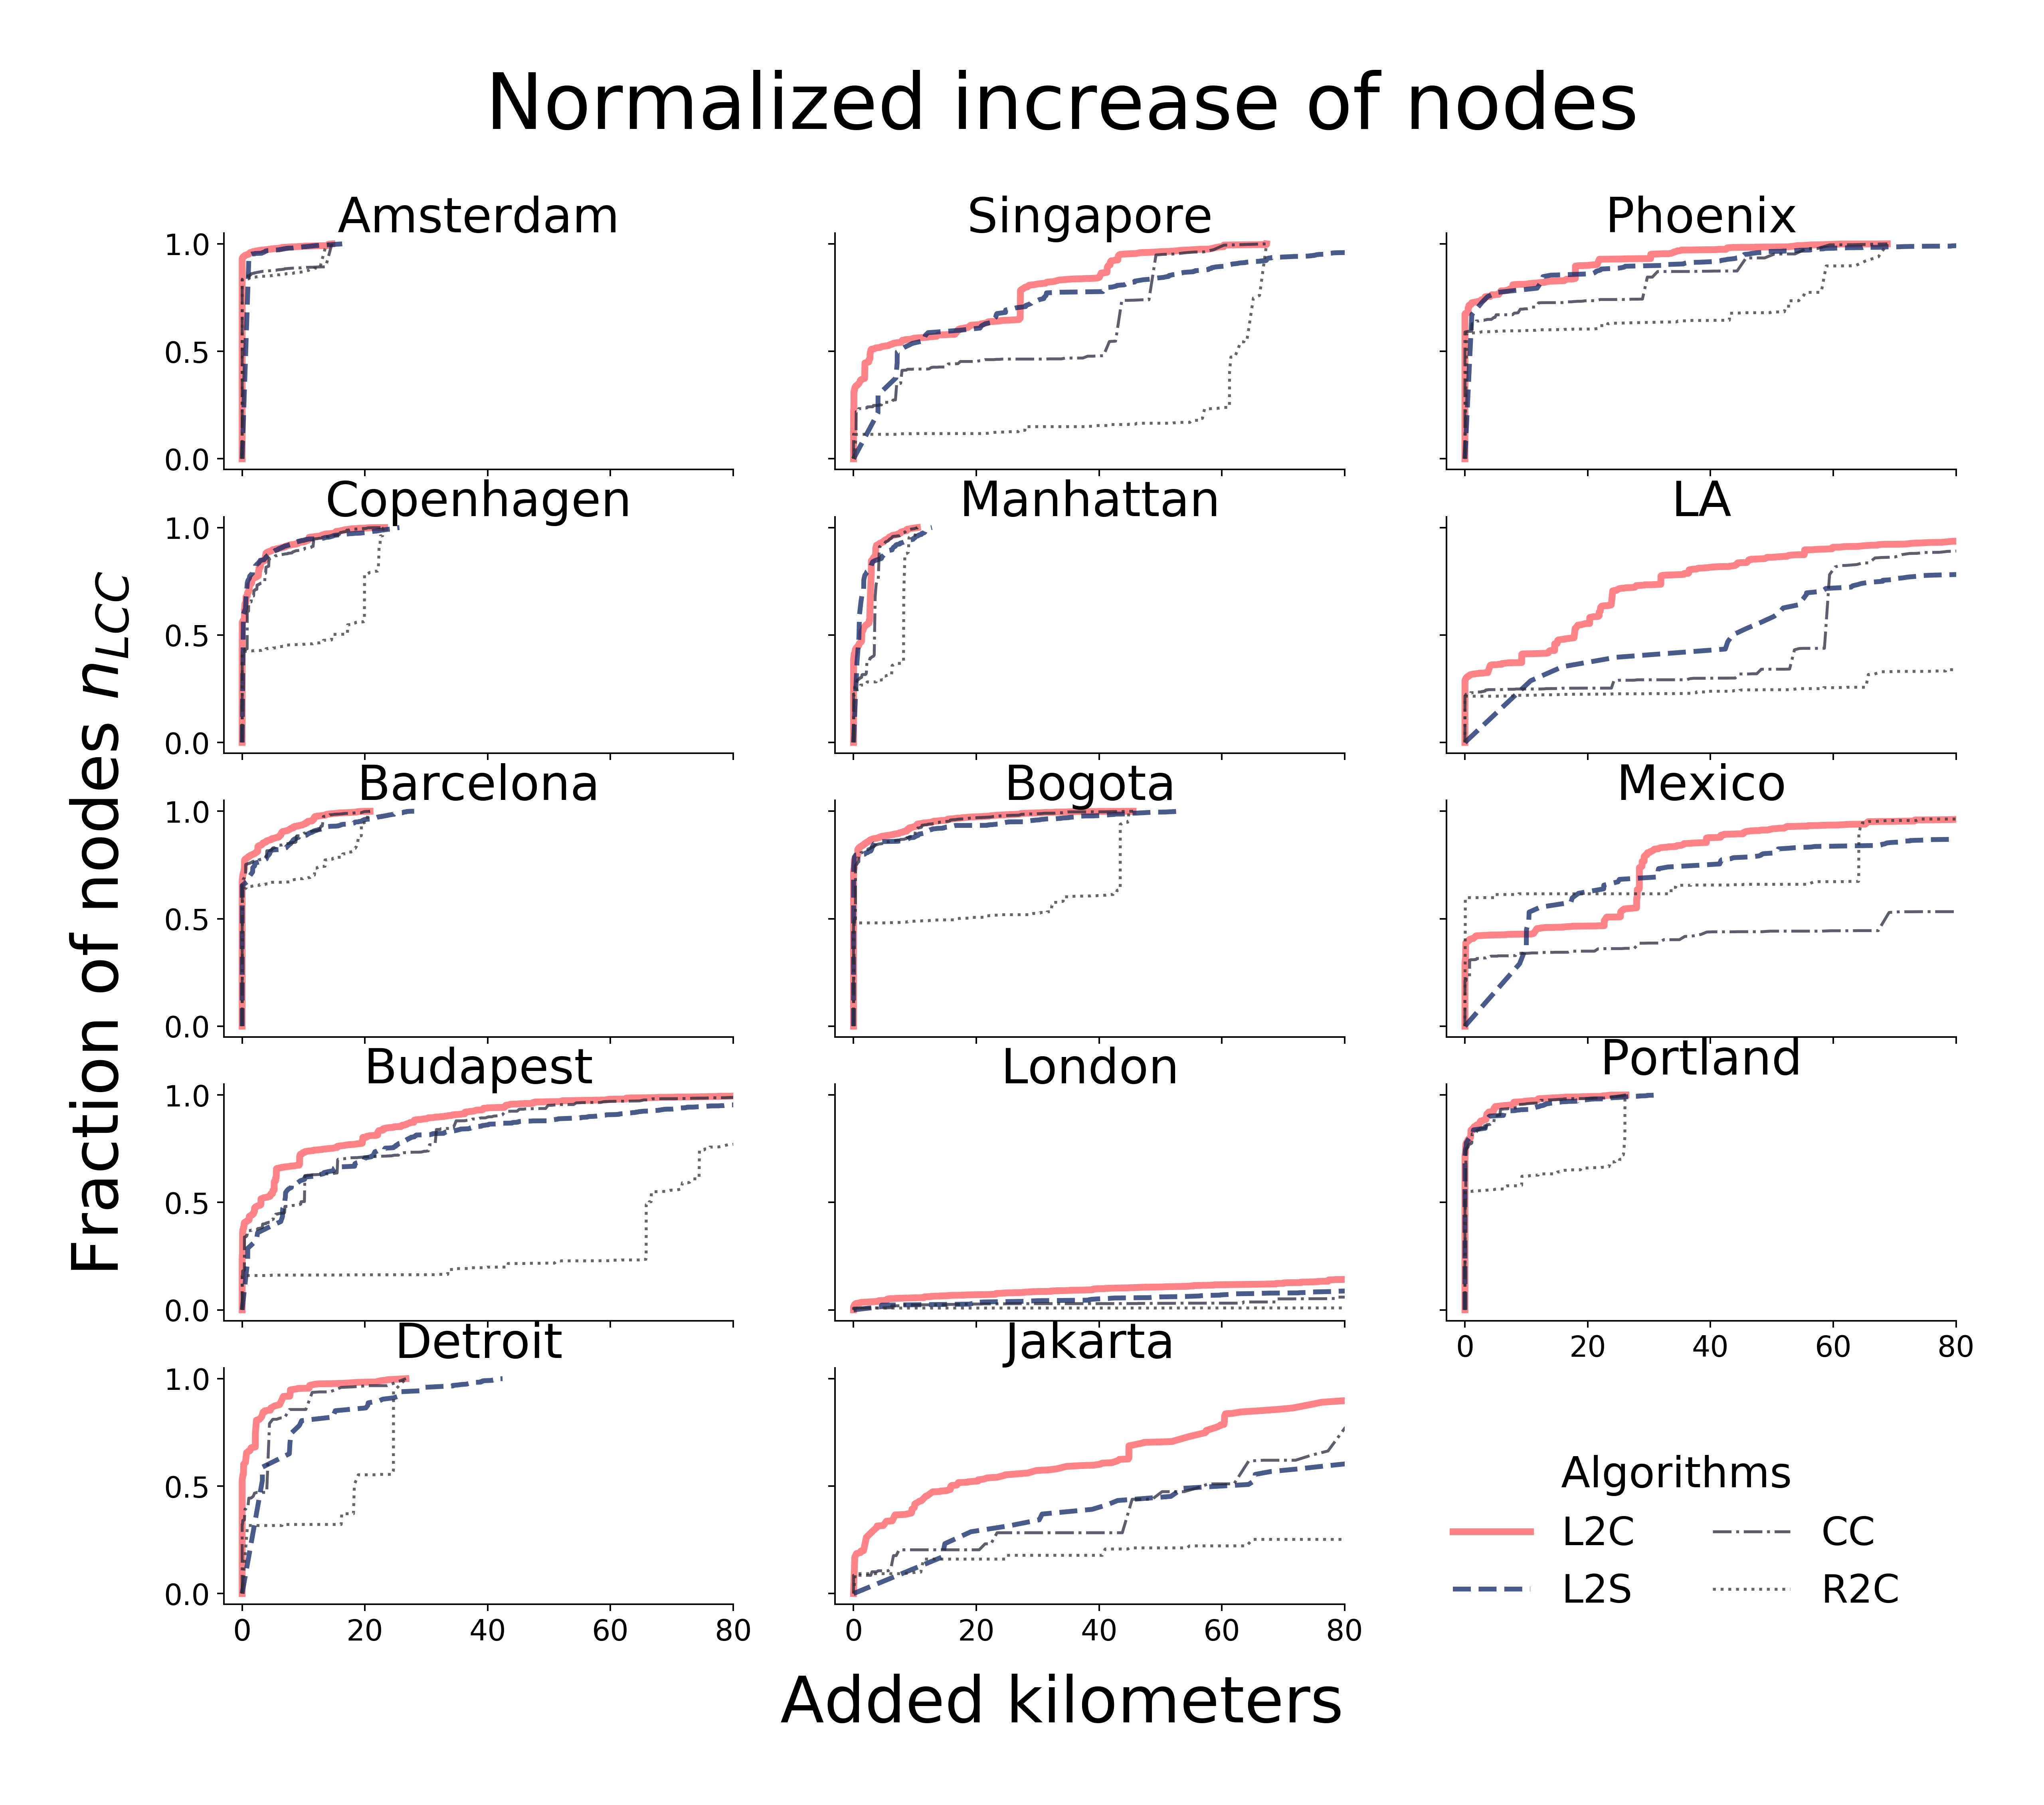
\includegraphics[width=0.8\textwidth]{images/datadriven/SI_Nodes_Bike_Streets.png}
  \caption{Normalized increase in nodes inside the largest connected component ($n_{LCC}$).}
  \label{fig:NodesIncrease_BikeStreets}
\end{figure*}

% \begin{figure*}[h!]
%   \centering
%   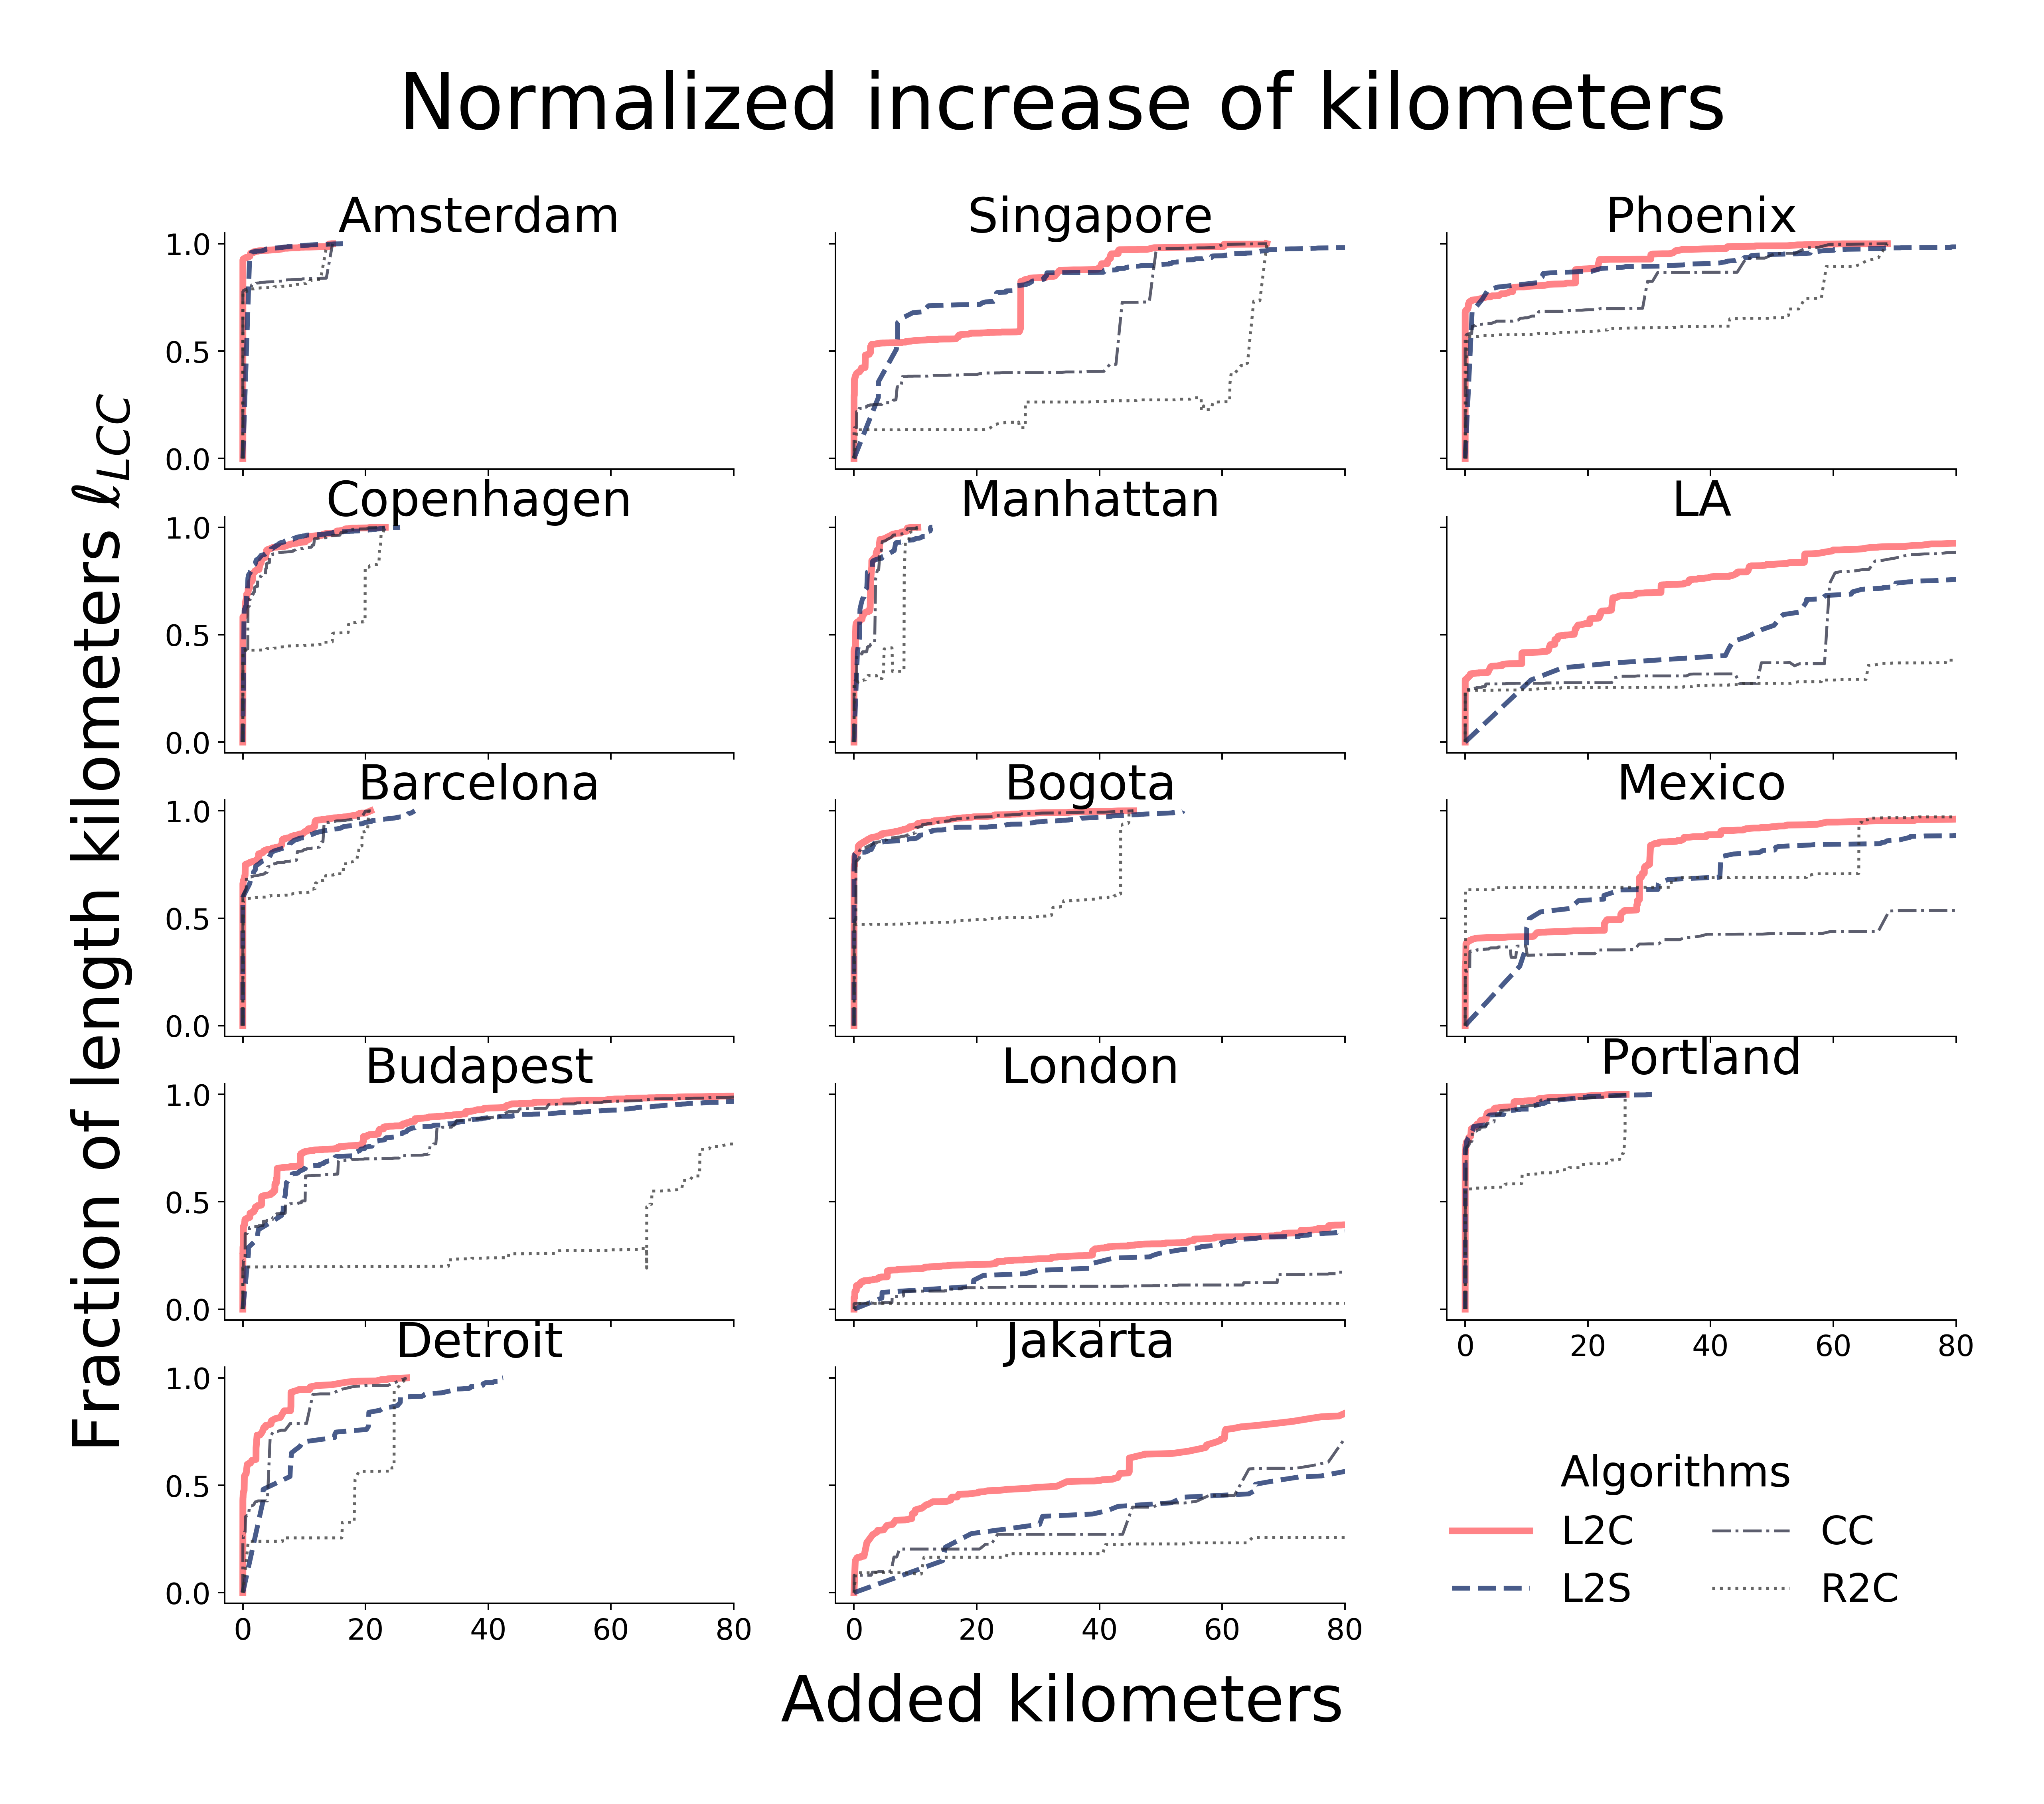
\includegraphics[width=0.8\textwidth]{images/datadriven/SI_Lengths_Bike_Streets.png}
%   \caption{Normalized increase in kilometers inside the largest connected component ($\ell_{LCC}$).}
%   \label{fig:Lengthsncrease_BikeStreets}
% \end{figure*}

\begin{figure*}[h!]
  \centering
  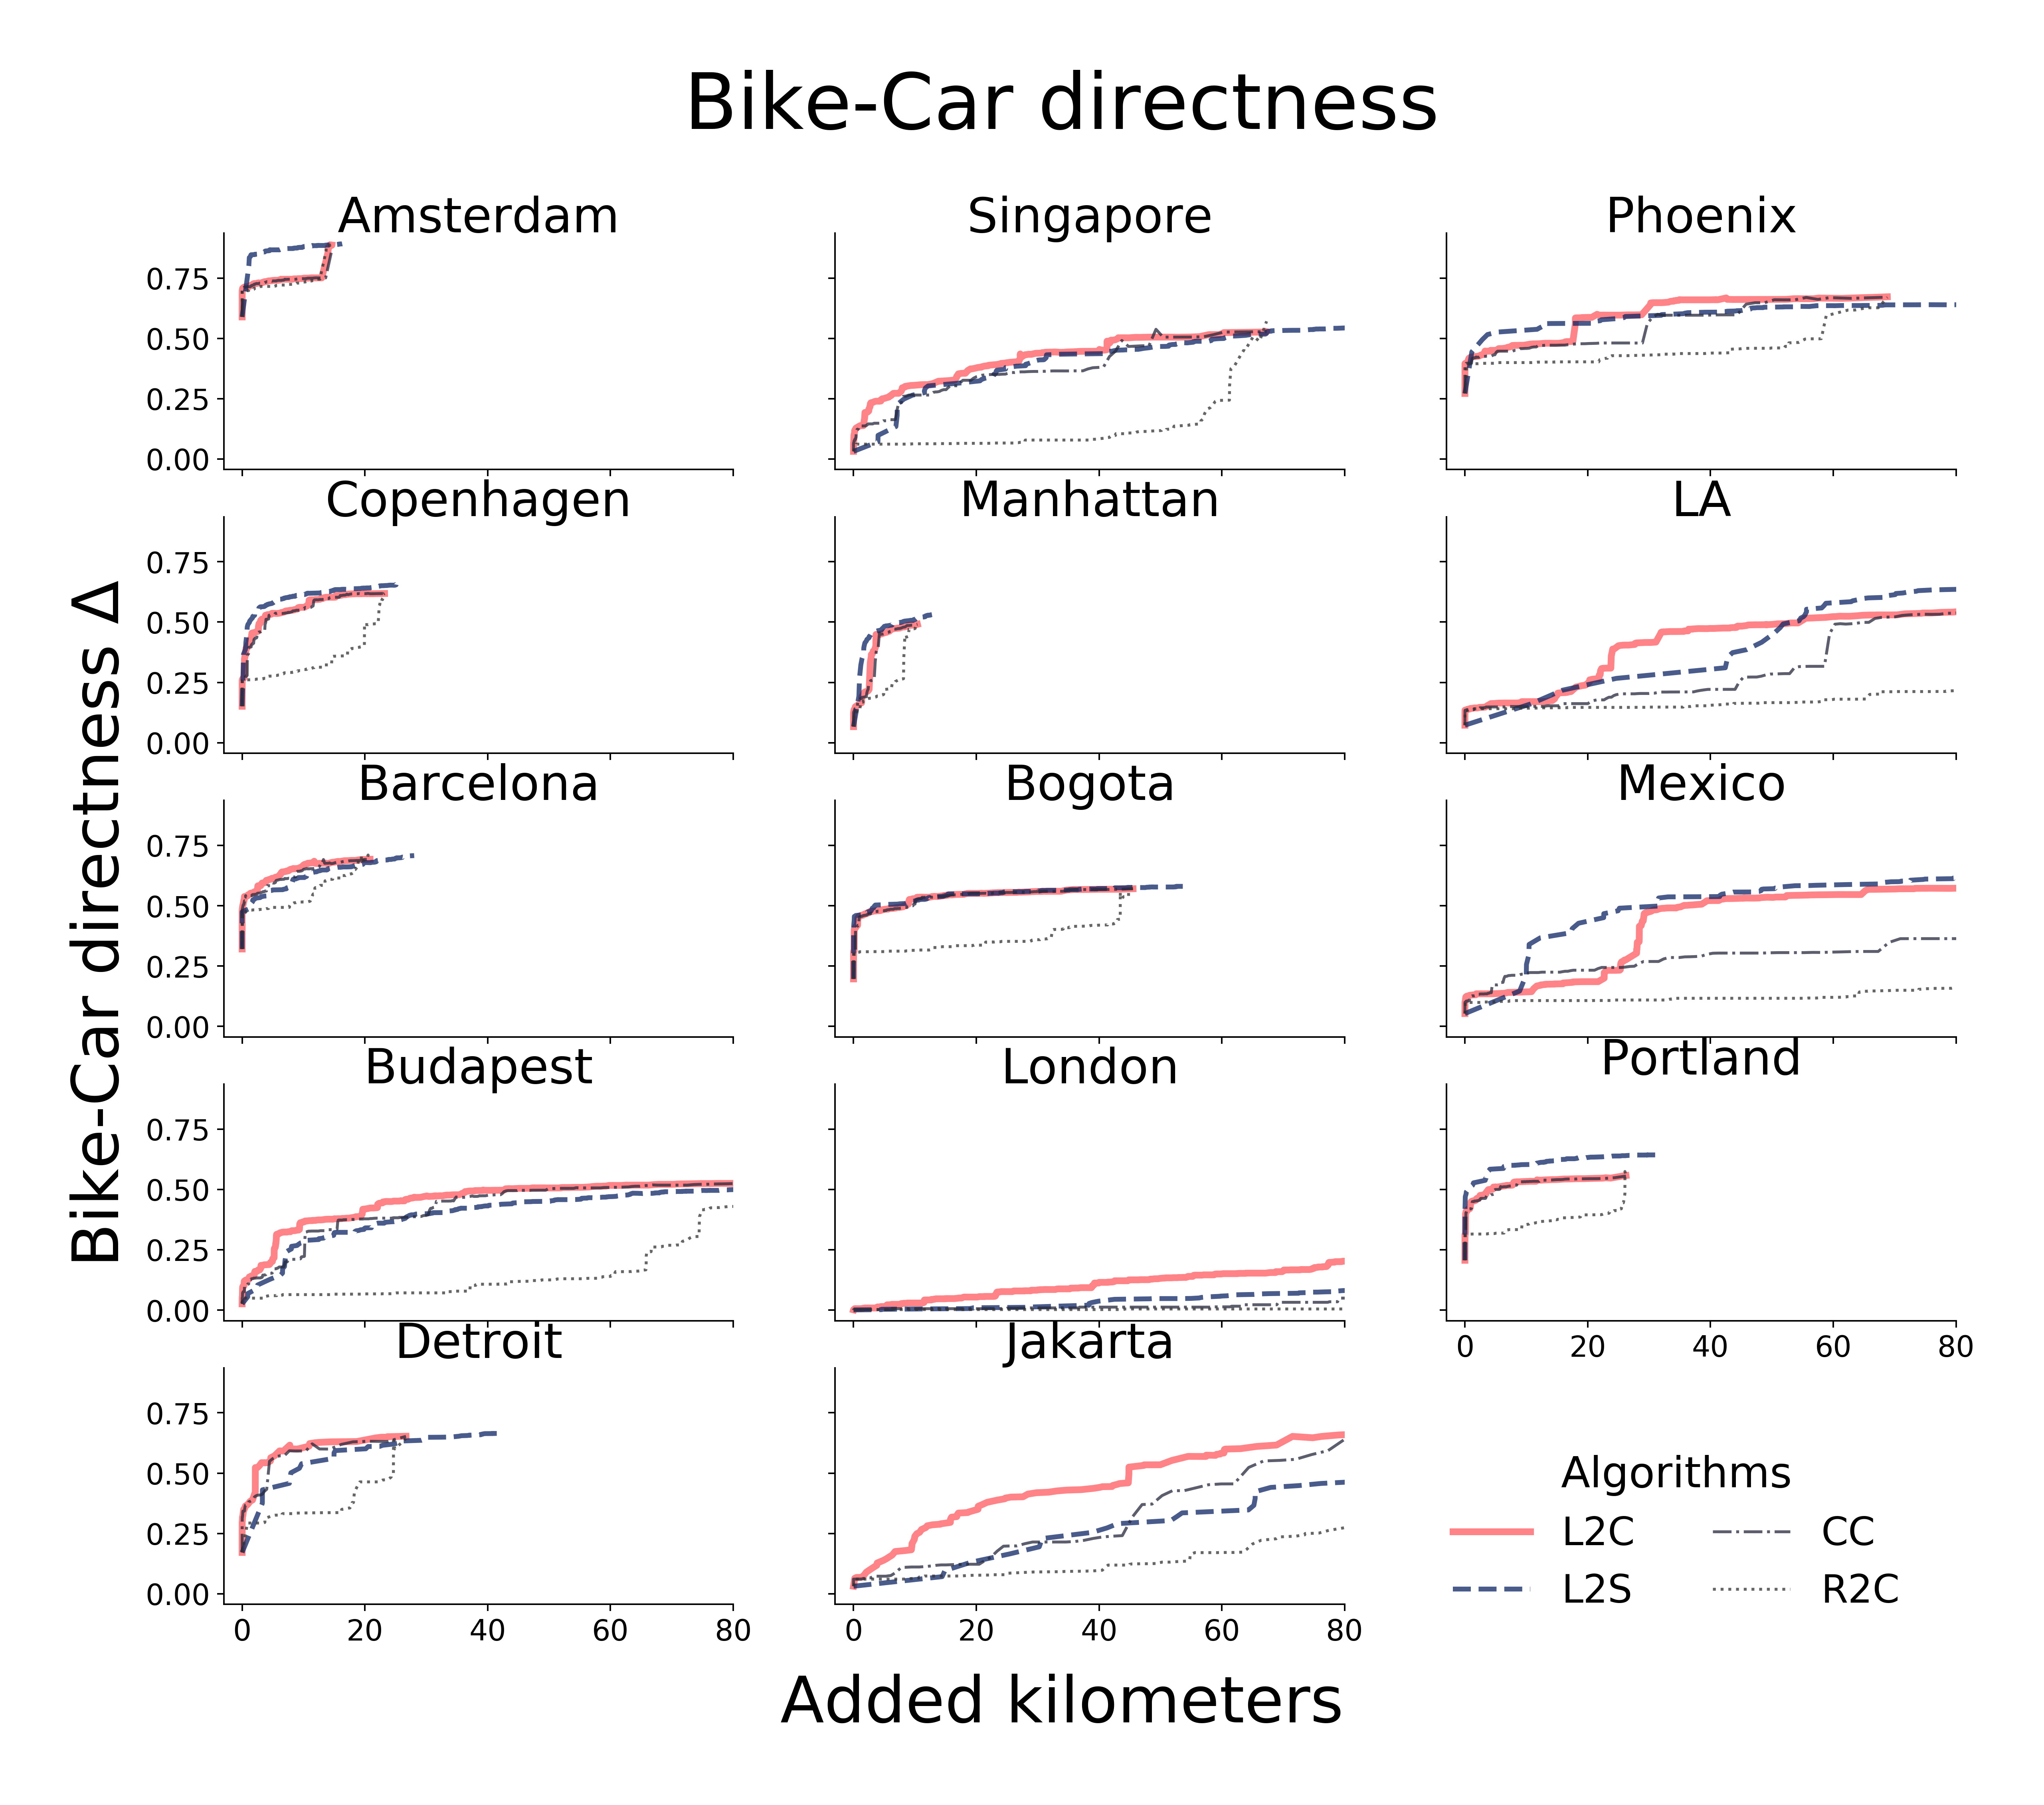
\includegraphics[width=0.8\textwidth]{images/datadriven/SI_Directness_Bike_Streets.png}
  \caption{Bike-car directness $\Delta$ per invested kilometers.}
  \label{fig:Directness_BikeStreets}
\end{figure*}

\begin{figure*}[h!]
  \centering
  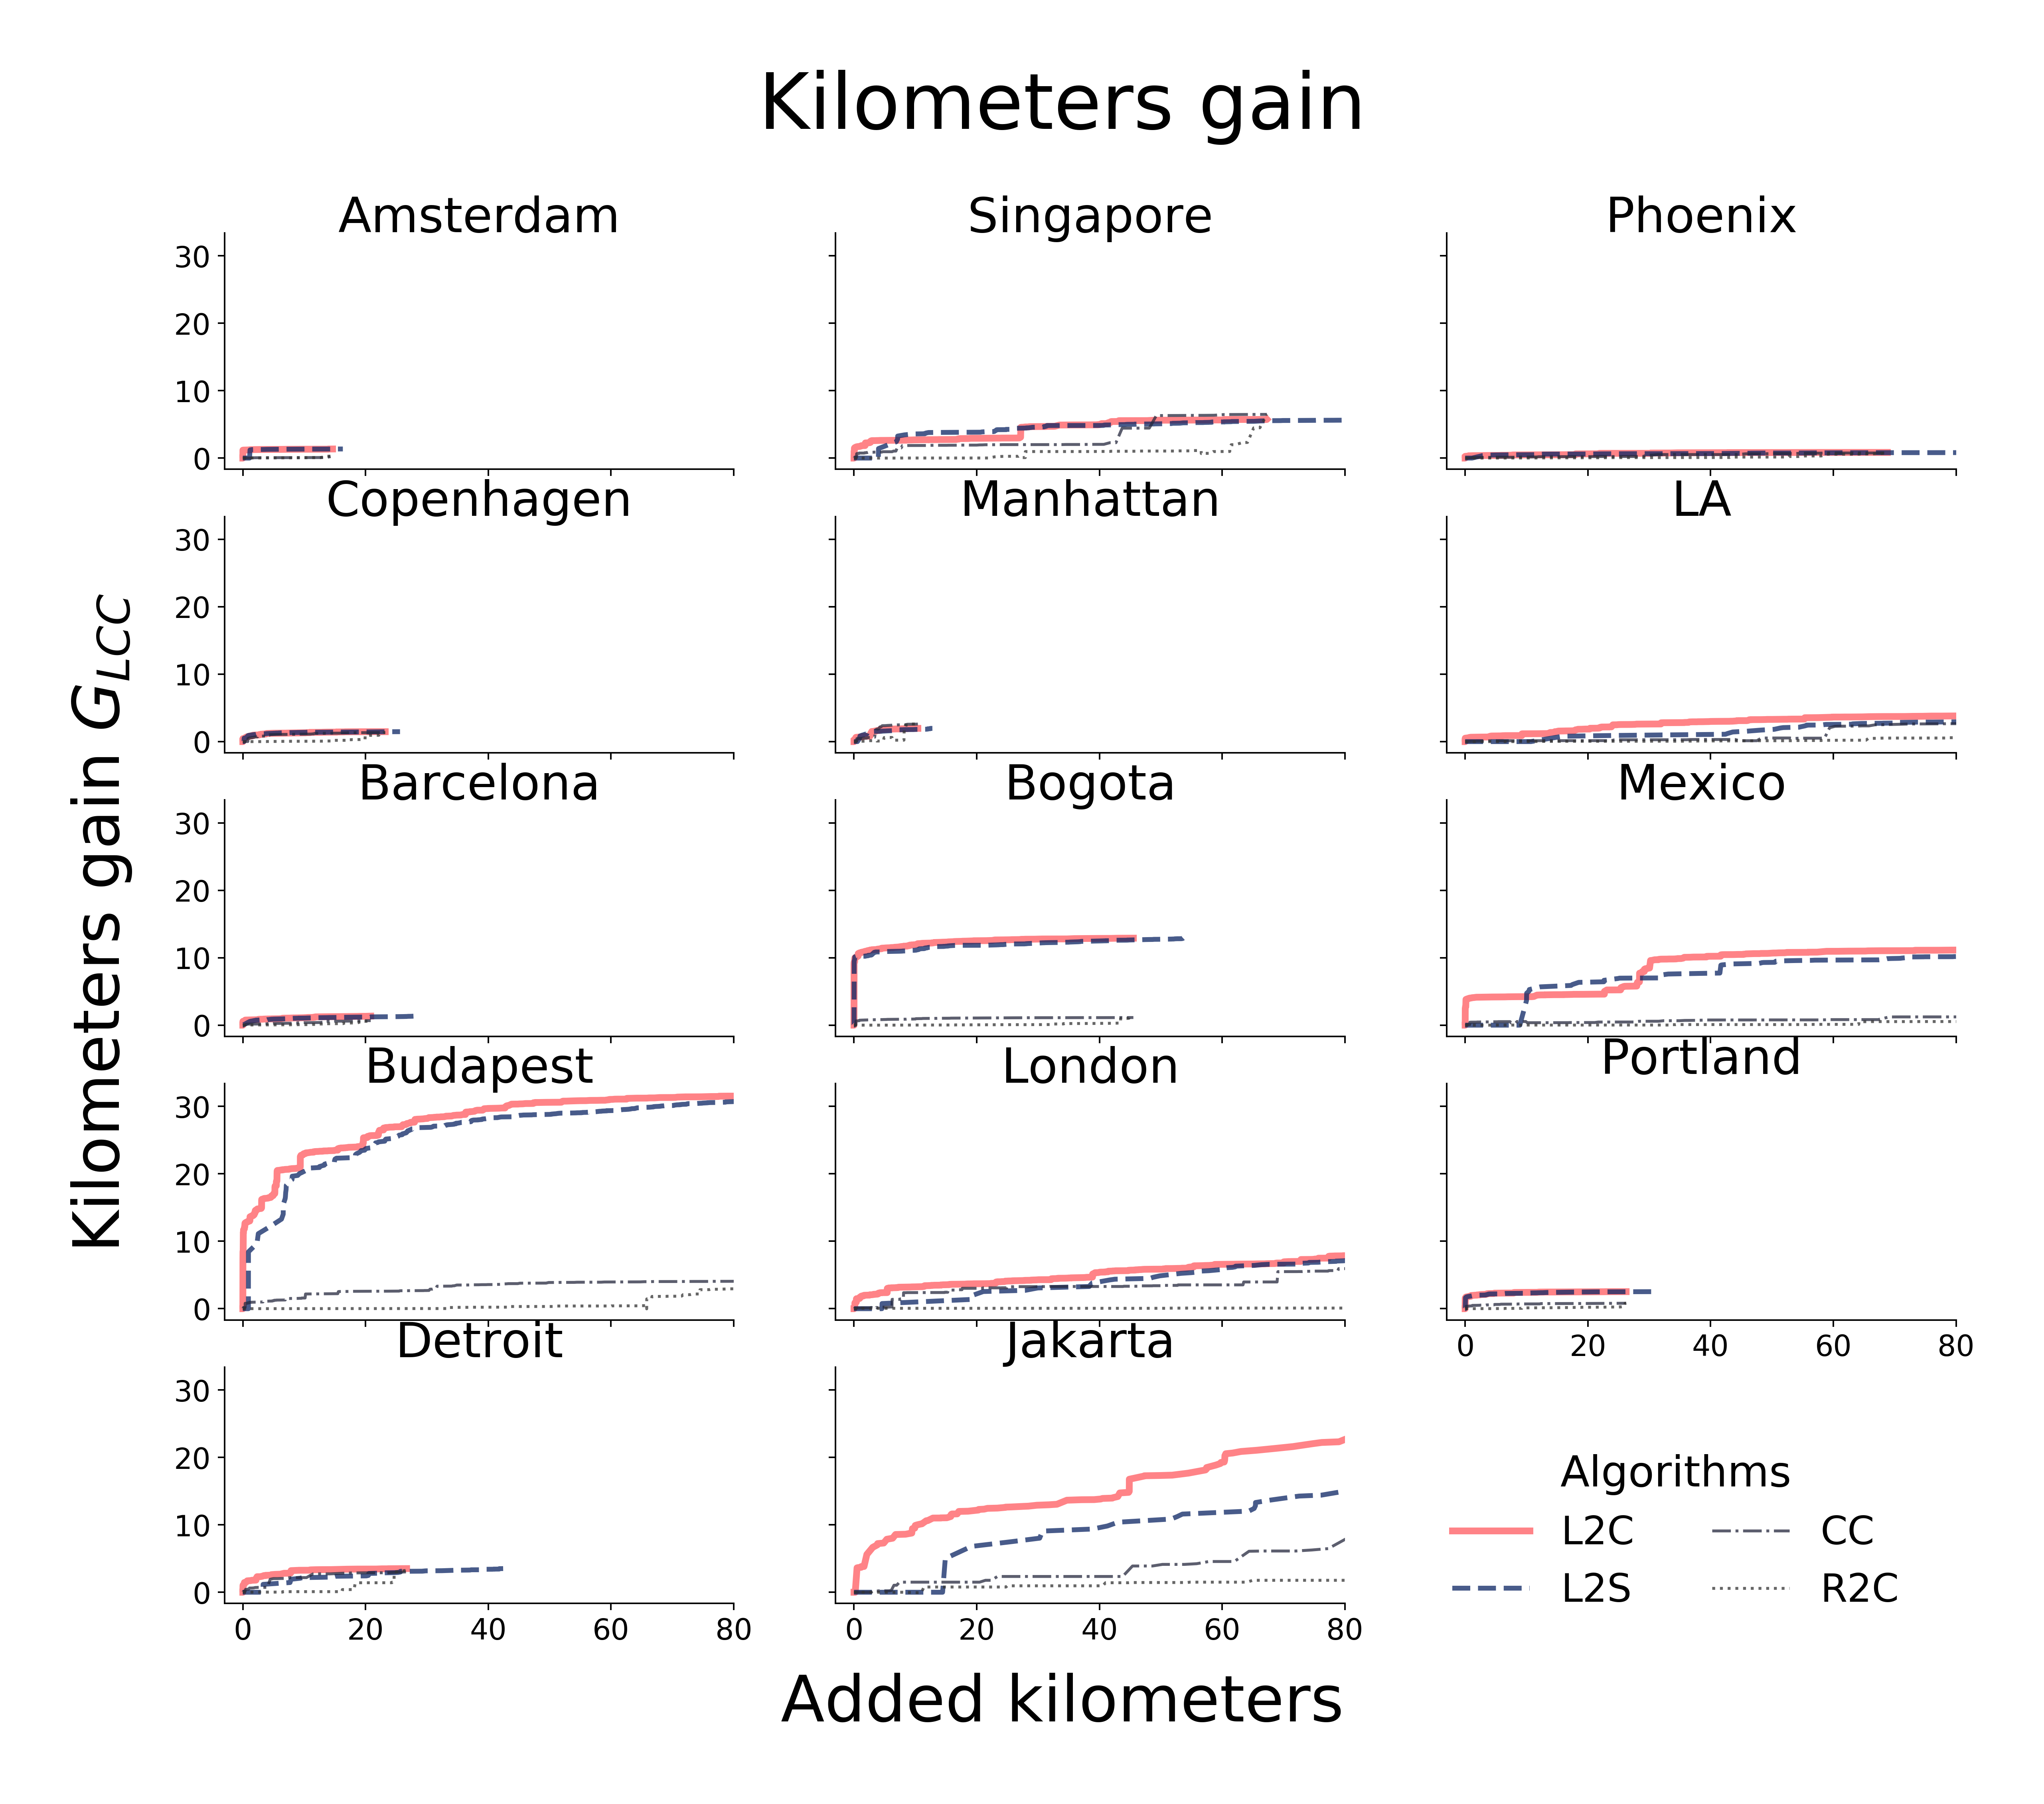
\includegraphics[width=0.8\textwidth]{images/datadriven/SI_Gain_Bike_Streets.png}
  \caption{Kilometers gain in the largest connected component.}
  \label{fig:Gain_BikeStreets}
\end{figure*}